\documentclass[paper=letter,11pt]{scrartcl}

\KOMAoptions{headinclude=true, footinclude=false}
\KOMAoptions{DIV=14, BCOR=5mm}
\KOMAoptions{numbers=noendperiod}
\KOMAoptions{parskip=half}
\addtokomafont{disposition}{\rmfamily}
\addtokomafont{part}{\LARGE}
\addtokomafont{descriptionlabel}{\rmfamily}
%\setkomafont{pageheadfoot}{\normalsize\sffamily}
\setkomafont{pagehead}{\normalsize\rmfamily}
%\setkomafont{publishers}{\normalsize\rmfamily}
\setkomafont{caption}{\normalfont\small}
\setcapindent{0pt}
\deffootnote[1em]{1em}{1em}{\textsuperscript{\thefootnotemark}\ }


\usepackage{amsmath}
\usepackage[varg]{txfonts}
\usepackage[T1]{fontenc}
\usepackage{graphicx}
\usepackage{xcolor}
\usepackage[american]{babel}
% hyperref is needed in many places, so include it here
\usepackage{hyperref}

\usepackage{xspace}
\usepackage{multirow}
\usepackage{float}


\usepackage{braket}
\usepackage{bbm}
\usepackage{relsize}
\usepackage{tcolorbox}

\def\ketY{\ensuremath{\ket {\Psi}}}
\def\iGeV{\ensuremath{\textrm{GeV}^{-1}}}
%\def\mp{\ensuremath{m_{\textrm{proton}}}}
\def\rp{\ensuremath{r_{\textrm{proton}}}}
\def\me{\ensuremath{m_{\textrm{electron}}}}
\def\aG{\ensuremath{\alpha_G}}
\def\rAtom{\ensuremath{r_{\textrm{atom}}}}
\def\rNucl{\ensuremath{r_{\textrm{nucleus}}}}
\def\GN{\ensuremath{\textrm{G}_\textrm{N}}}
\def\ketX{\ensuremath{\ket{\vec{x}}}}
\def\ve{\ensuremath{\vec{\epsilon}}}


\def\ABCDMatrix{\ensuremath{\begin{pmatrix} A &  B  \\ C  & D \end{pmatrix}}}
\def\xyprime{\ensuremath{\begin{pmatrix} x' \\ y' \end{pmatrix}}}
\def\xyprimeT{\ensuremath{\begin{pmatrix} x' &  y' \end{pmatrix}}}
\def\xy{\ensuremath{\begin{pmatrix} x \\ y \end{pmatrix}}}
\def\xyT{\ensuremath{\begin{pmatrix} x & y \end{pmatrix}}}

\def\IMatrix{\ensuremath{\begin{pmatrix} 0 &  1  \\ -1  & 0 \end{pmatrix}}}
\def\IBoostMatrix{\ensuremath{\begin{pmatrix} 0 &  1  \\ 1  & 0 \end{pmatrix}}}
\def\JThree{\ensuremath{\begin{pmatrix}    0 & -i & 0  \\ i & 0  & 0 \\ 0 & 0 & 0 \end{pmatrix}}} 
\def\JTwo{\ensuremath{\begin{bmatrix}    0 & 0 & -i  \\ 0 & 0  & 0 \\ i & 0 & 0 \end{bmatrix}}}
\def\JOne{\ensuremath{\begin{bmatrix}    0 & 0 & 0  \\ 0 & 0  & -i \\ 0 & i & 0 \end{bmatrix}}}
\def\etamn{\ensuremath{\eta_{\mu\nu}}}
\def\Lmn{\ensuremath{\Lambda^\mu_\nu}}
\def\dmn{\ensuremath{\delta^\mu_\nu}}
\def\wmn{\ensuremath{\omega^\mu_\nu}}
\def\be{\begin{equation*}}
\def\ee{\end{equation*}}
\def\bea{\begin{eqnarray*}}
\def\eea{\end{eqnarray*}}
\def\bi{\begin{itemize}}
\def\ei{\end{itemize}}
\def\fmn{\ensuremath{F_{\mu\nu}}}
\def\fMN{\ensuremath{F^{\mu\nu}}}
\def\bc{\begin{center}}
\def\ec{\end{center}}
\def\nus{$\nu$s}

\def\adagger{\ensuremath{a_{p\sigma}^\dagger}}
\def\lineacross{\noindent\rule{\textwidth}{1pt}}

\newcommand{\multiline}[1] {
\begin{tabular} {|l}
#1
\end{tabular}
}

\newcommand{\multilineNoLine}[1] {
\begin{tabular} {l}
#1
\end{tabular}
}



\newcommand{\lineTwo}[2] {
\begin{tabular} {|l}
#1 \\
#2
\end{tabular}
}

\newcommand{\rmt}[1] {
\textrm{#1}
}


%
% Units
%
\def\m{\ensuremath{\rmt{m}}}
\def\GeV{\ensuremath{\rmt{GeV}}}
\def\pt{\ensuremath{p_\rmt{T}}}


\def\parity{\ensuremath{\mathcal{P}}}

\usepackage{cancel}
\usepackage{ mathrsfs }
\def\bigL{\ensuremath{\mathscr{L}}}

\usepackage{ dsfont }



\usepackage{fancyhdr}
\fancyhf{}


\lhead{\Large 33-444} % \hfill Introduction to Particle Physics \hfill Spring 2020}
\chead{\Large Introduction to Particle Physics} % \hfill Spring 2020}
\rhead{\Large Spring 2020} % \hfill Introduction to Particle Physics \hfill Spring 2020}

\begin{document}
\thispagestyle{fancy}

\begin{center}
{\huge \textbf{Lecture 25}}
\end{center}

{\fontsize{14}{16}\selectfont

\bc
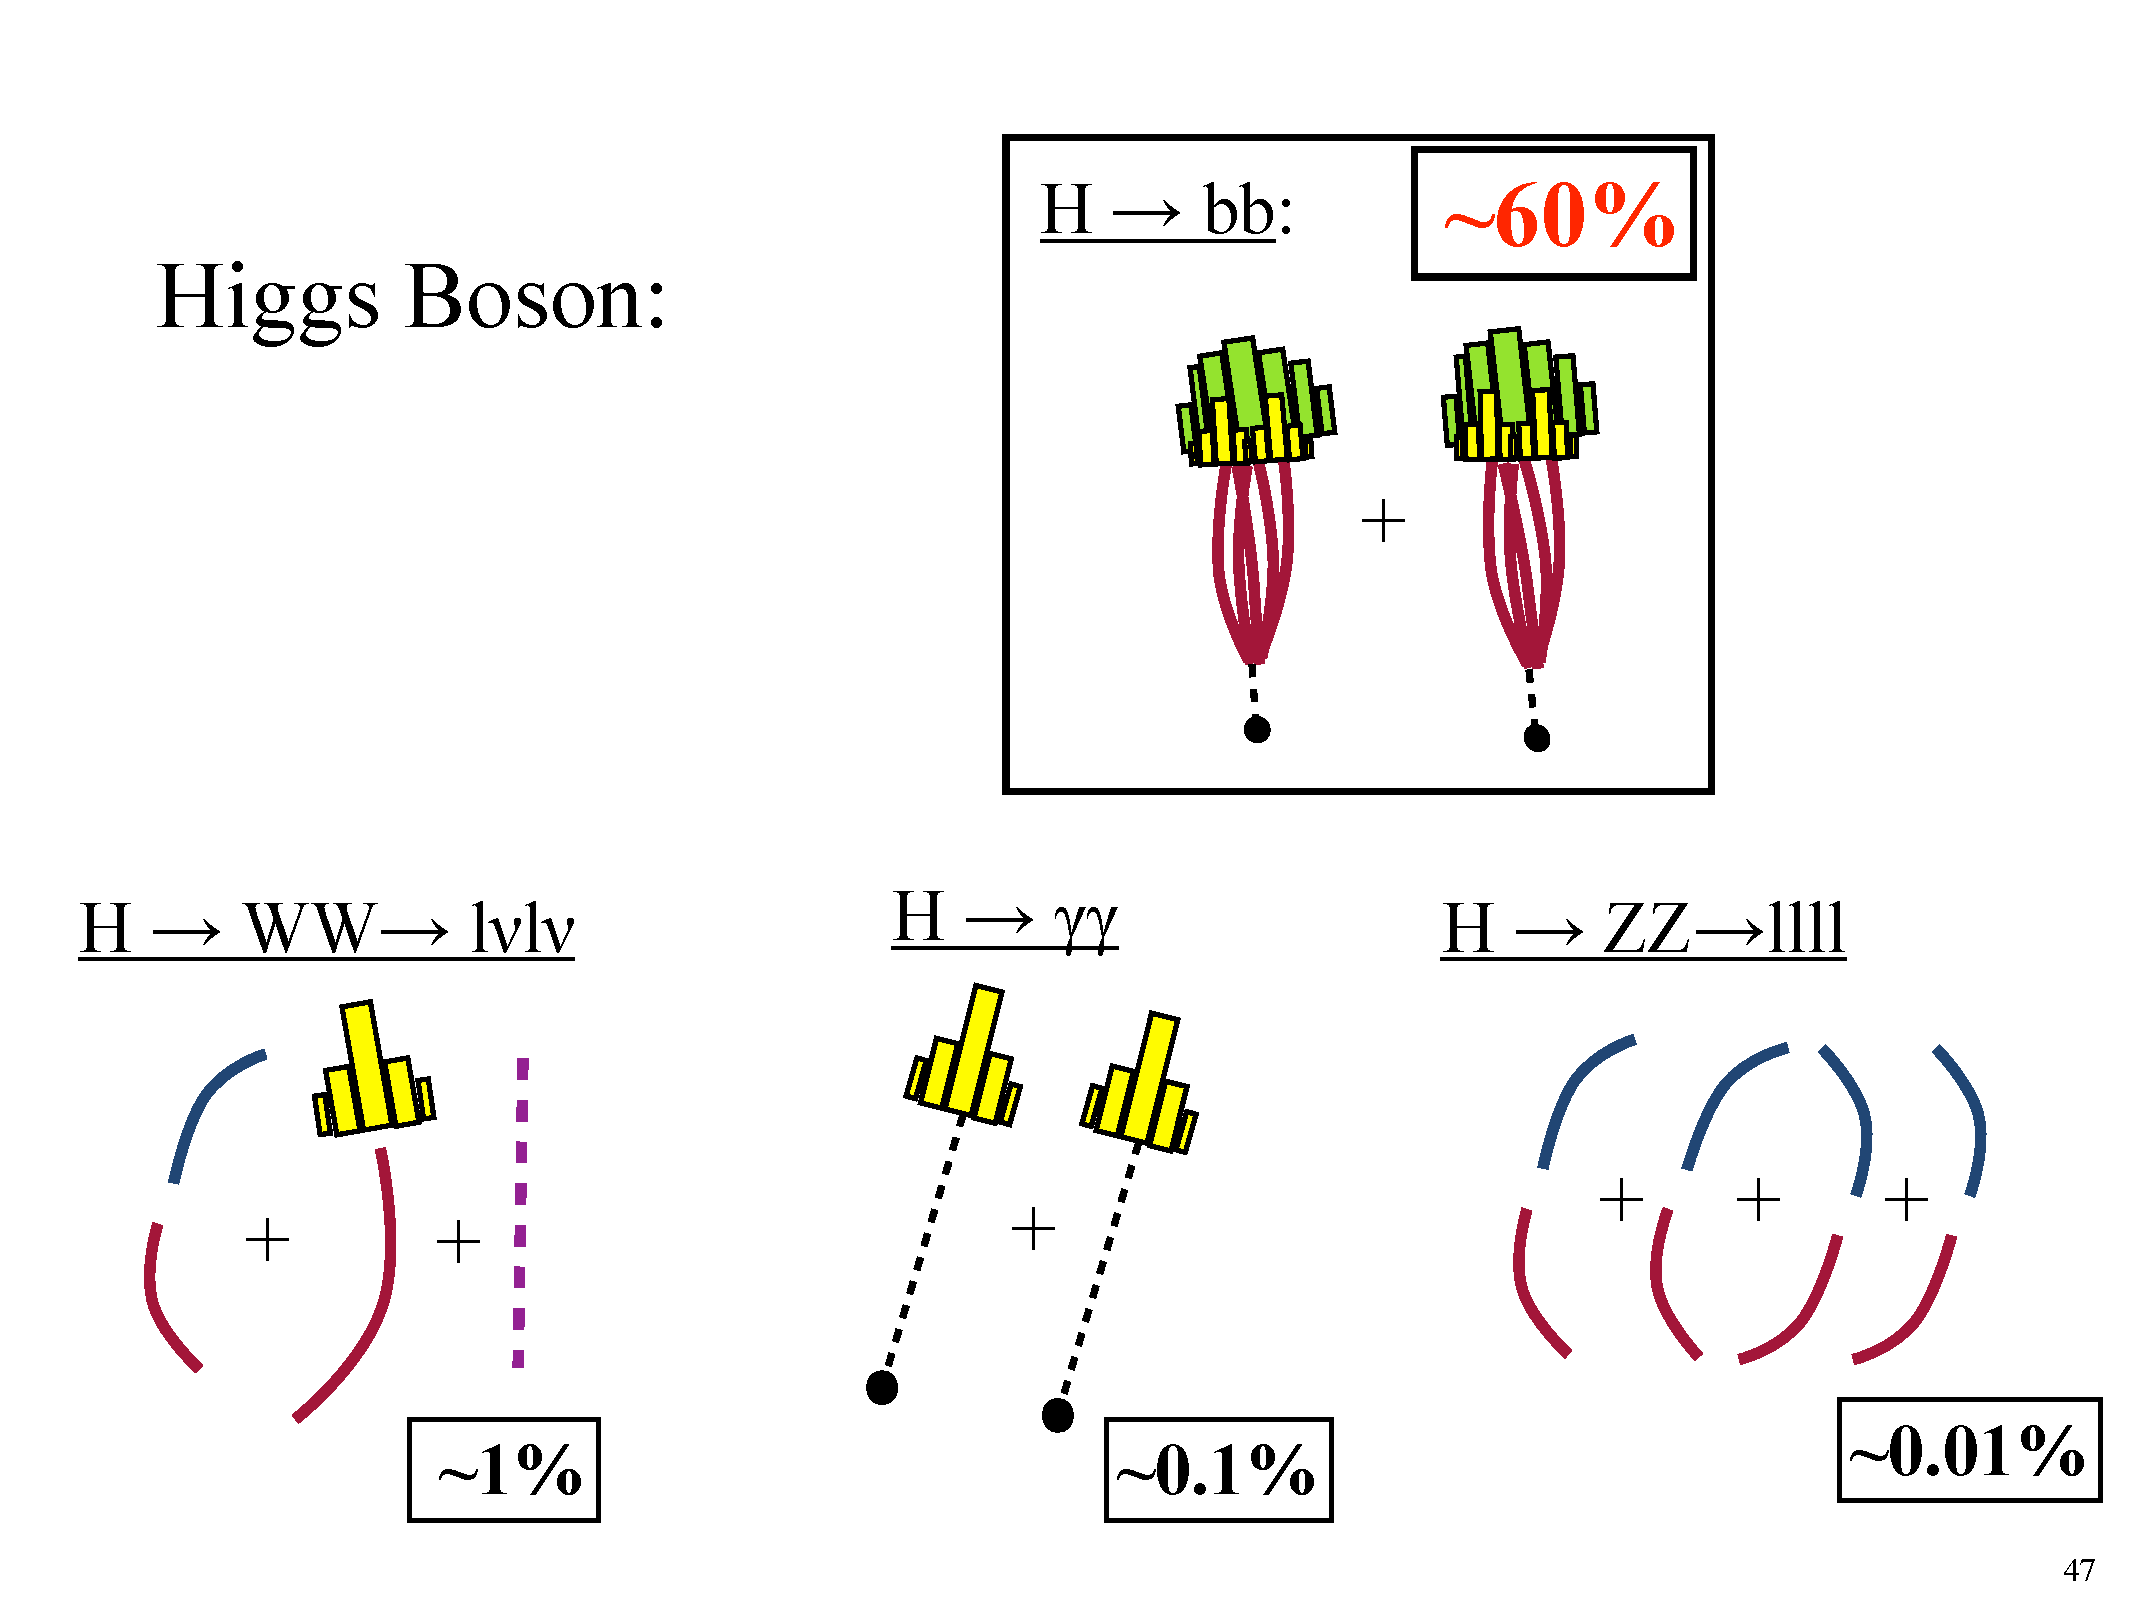
\includegraphics[width=0.725\textwidth]{./HiggsBosonDecays.pdf}
\ec
\lineacross
\bc
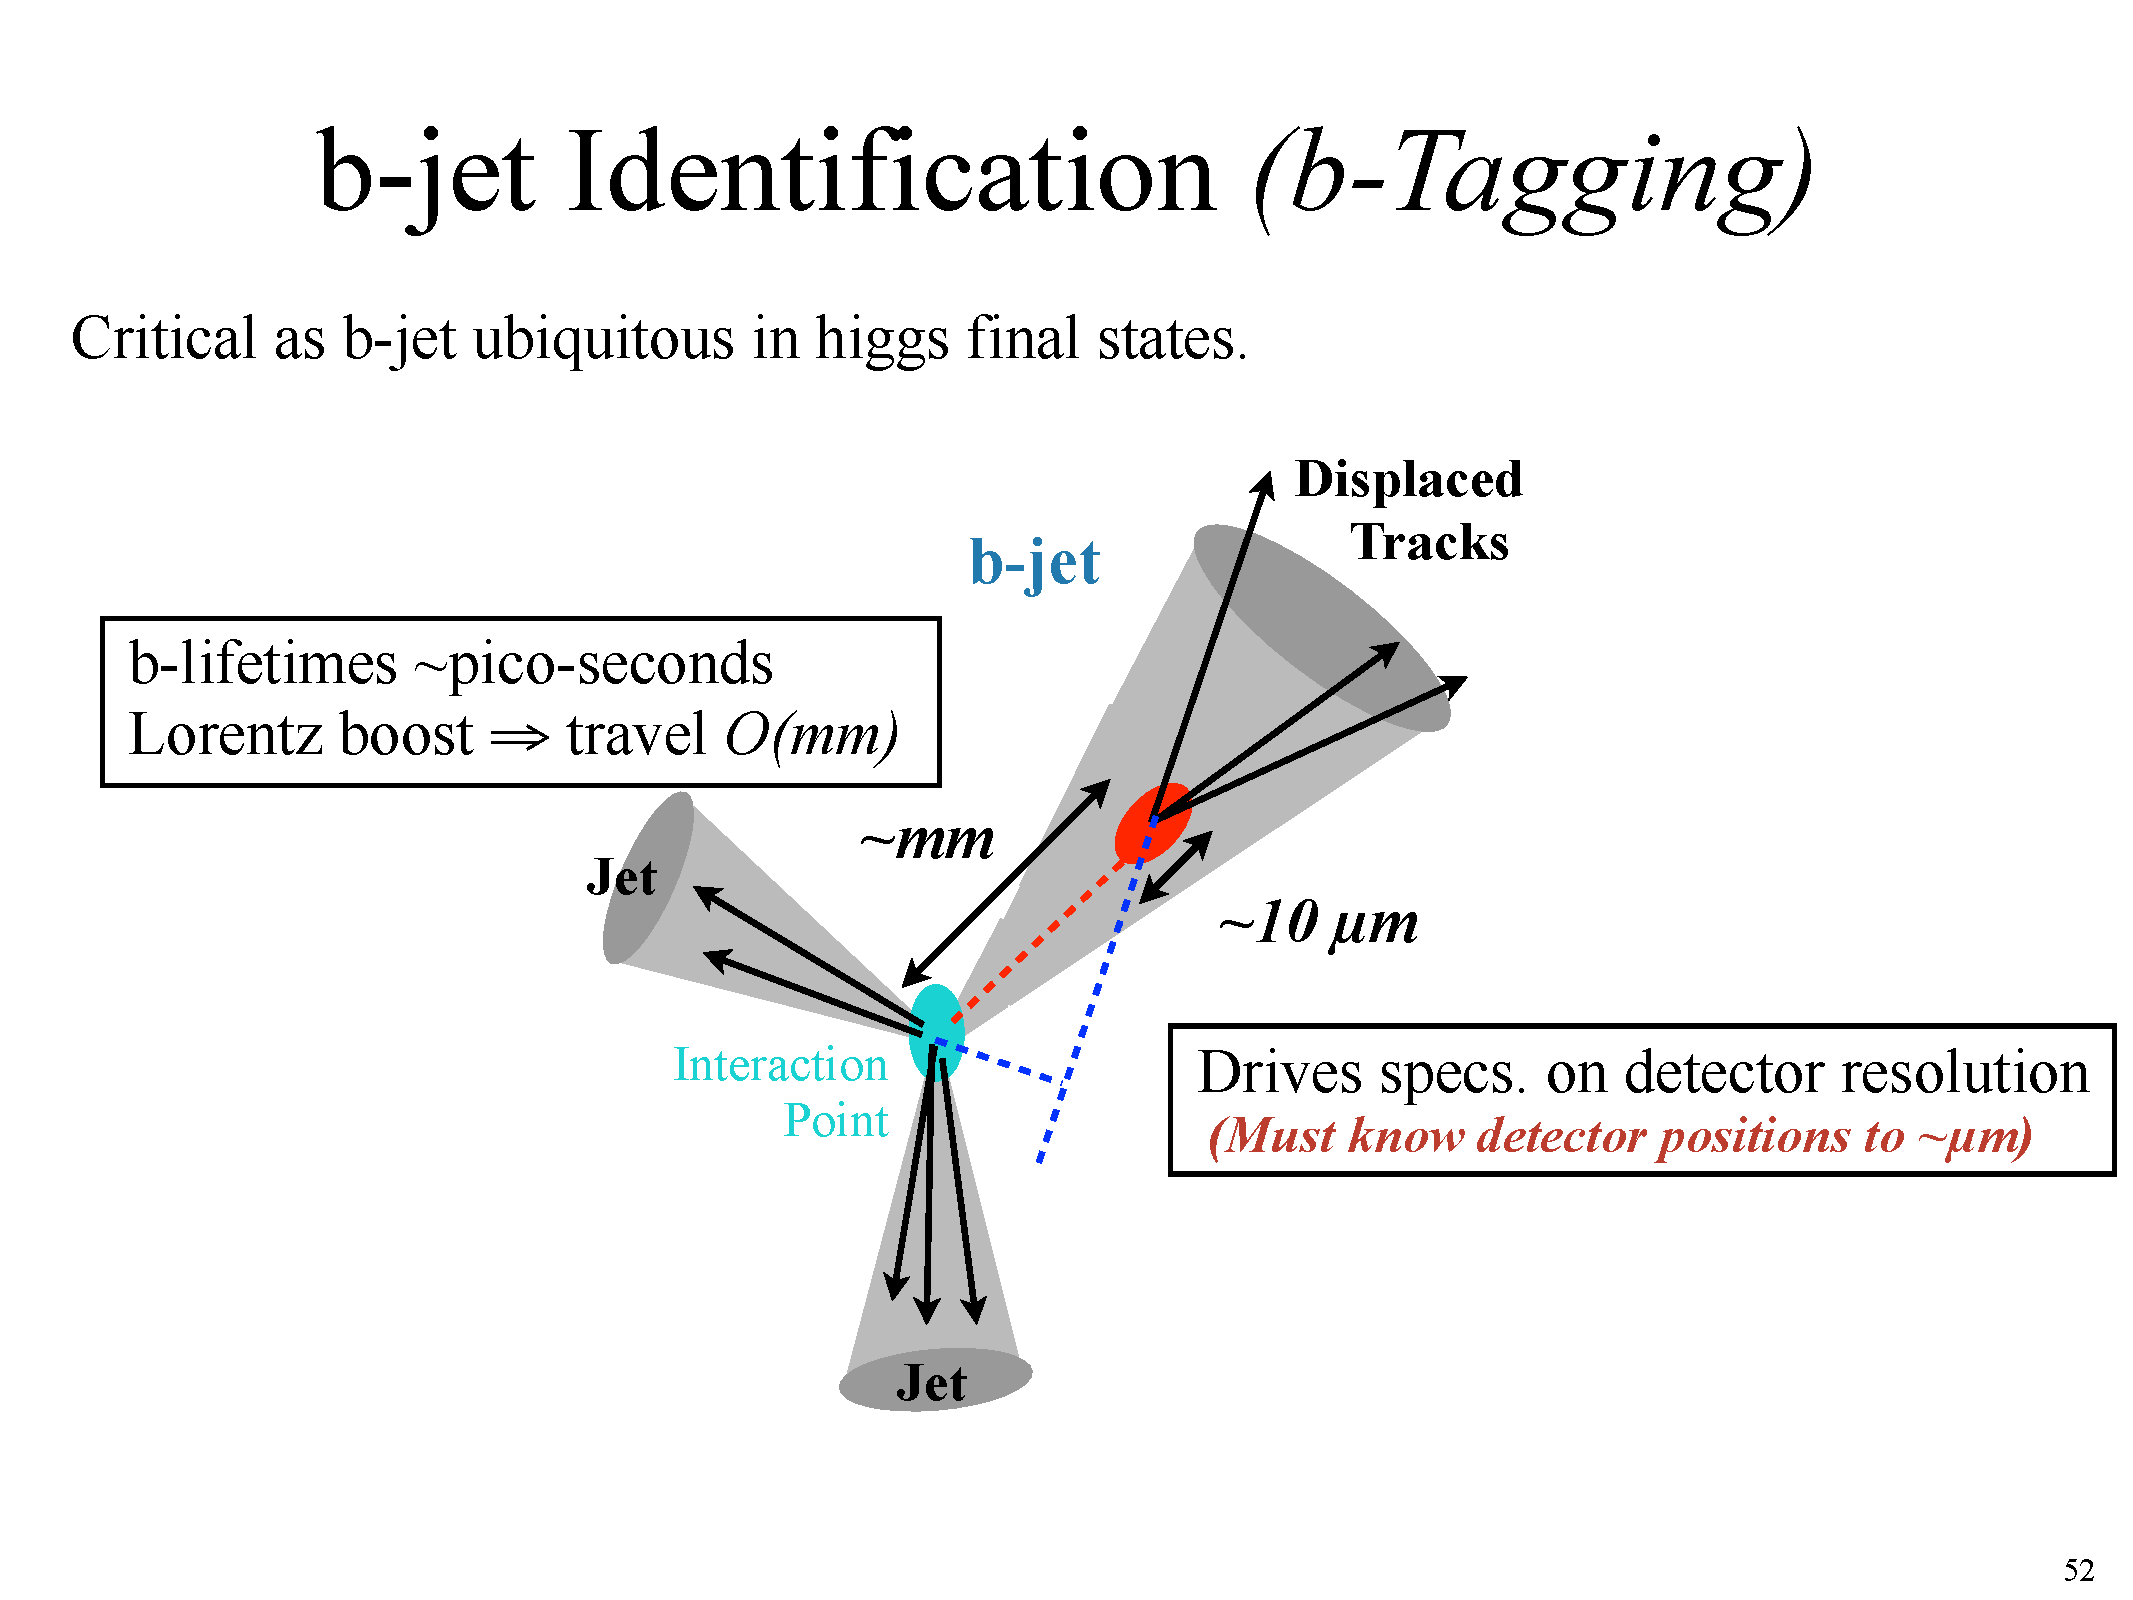
\includegraphics[width=0.725\textwidth]{./BTagging.pdf}
\ec

\clearpage

\bc
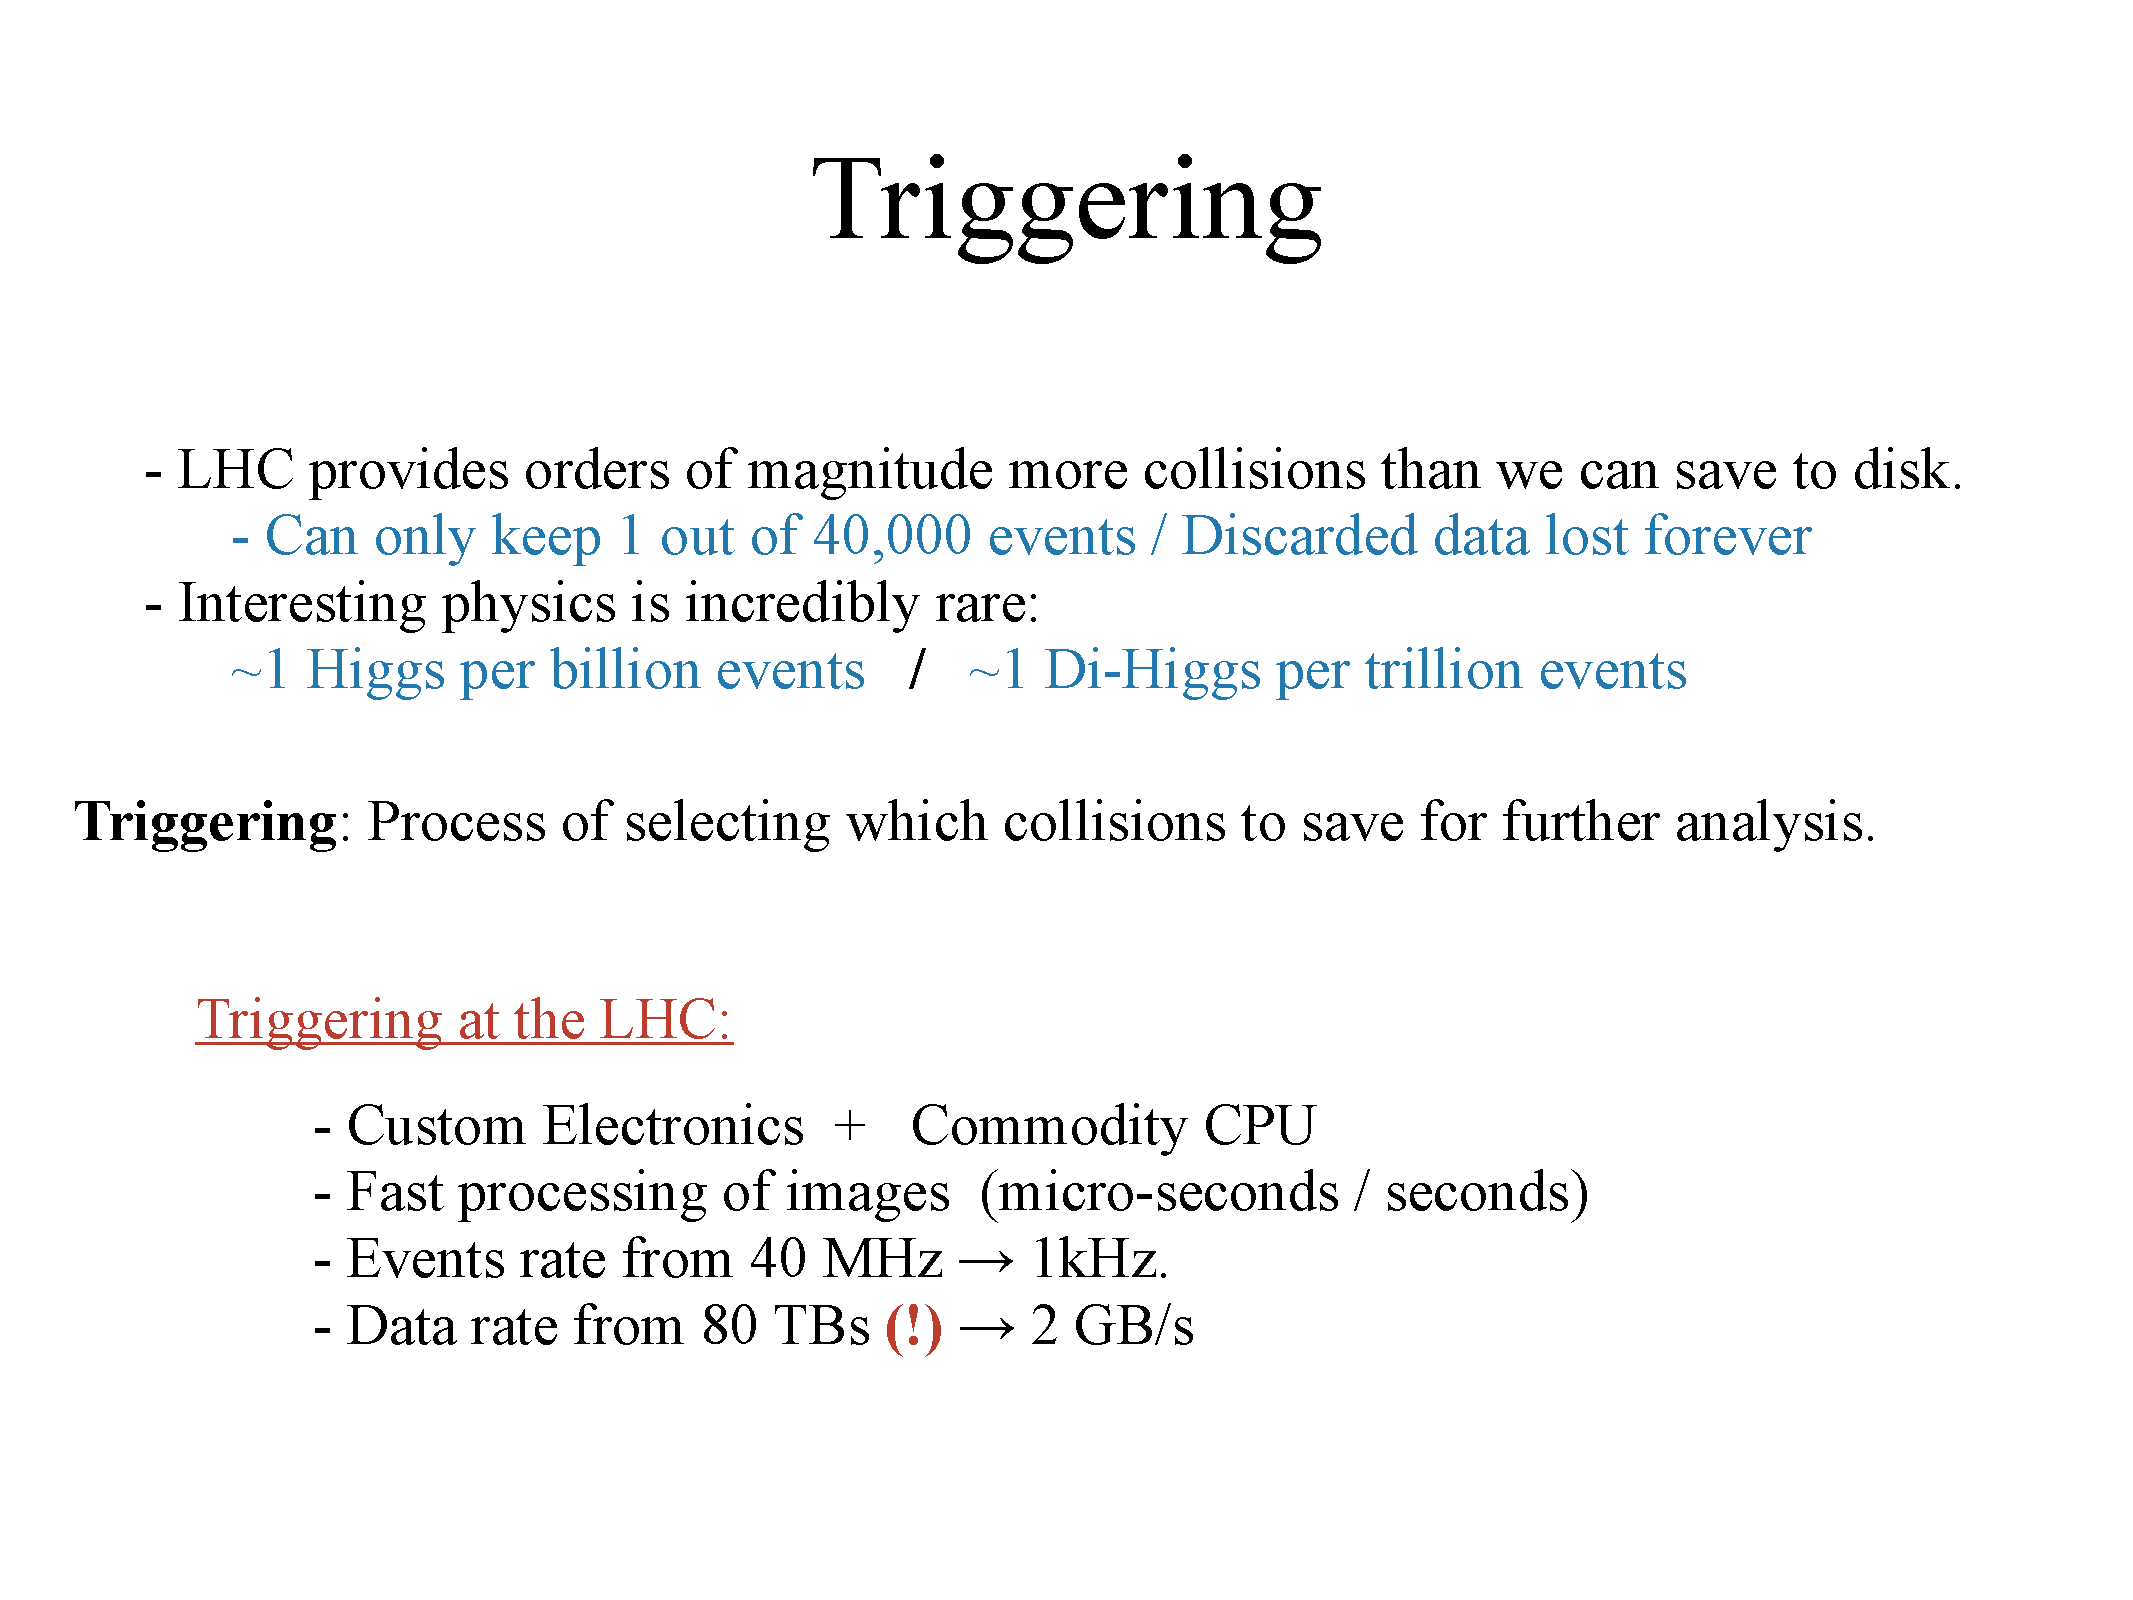
\includegraphics[width=0.725\textwidth]{./Triggering.pdf}
\ec
\lineacross

To collect data faster, each event has multiple proton collisions.

Significantly complicates analysis of events
\bc
\includegraphics[width=0.725\textwidth]{./NoPileUp.pdf}
\ec


\bc
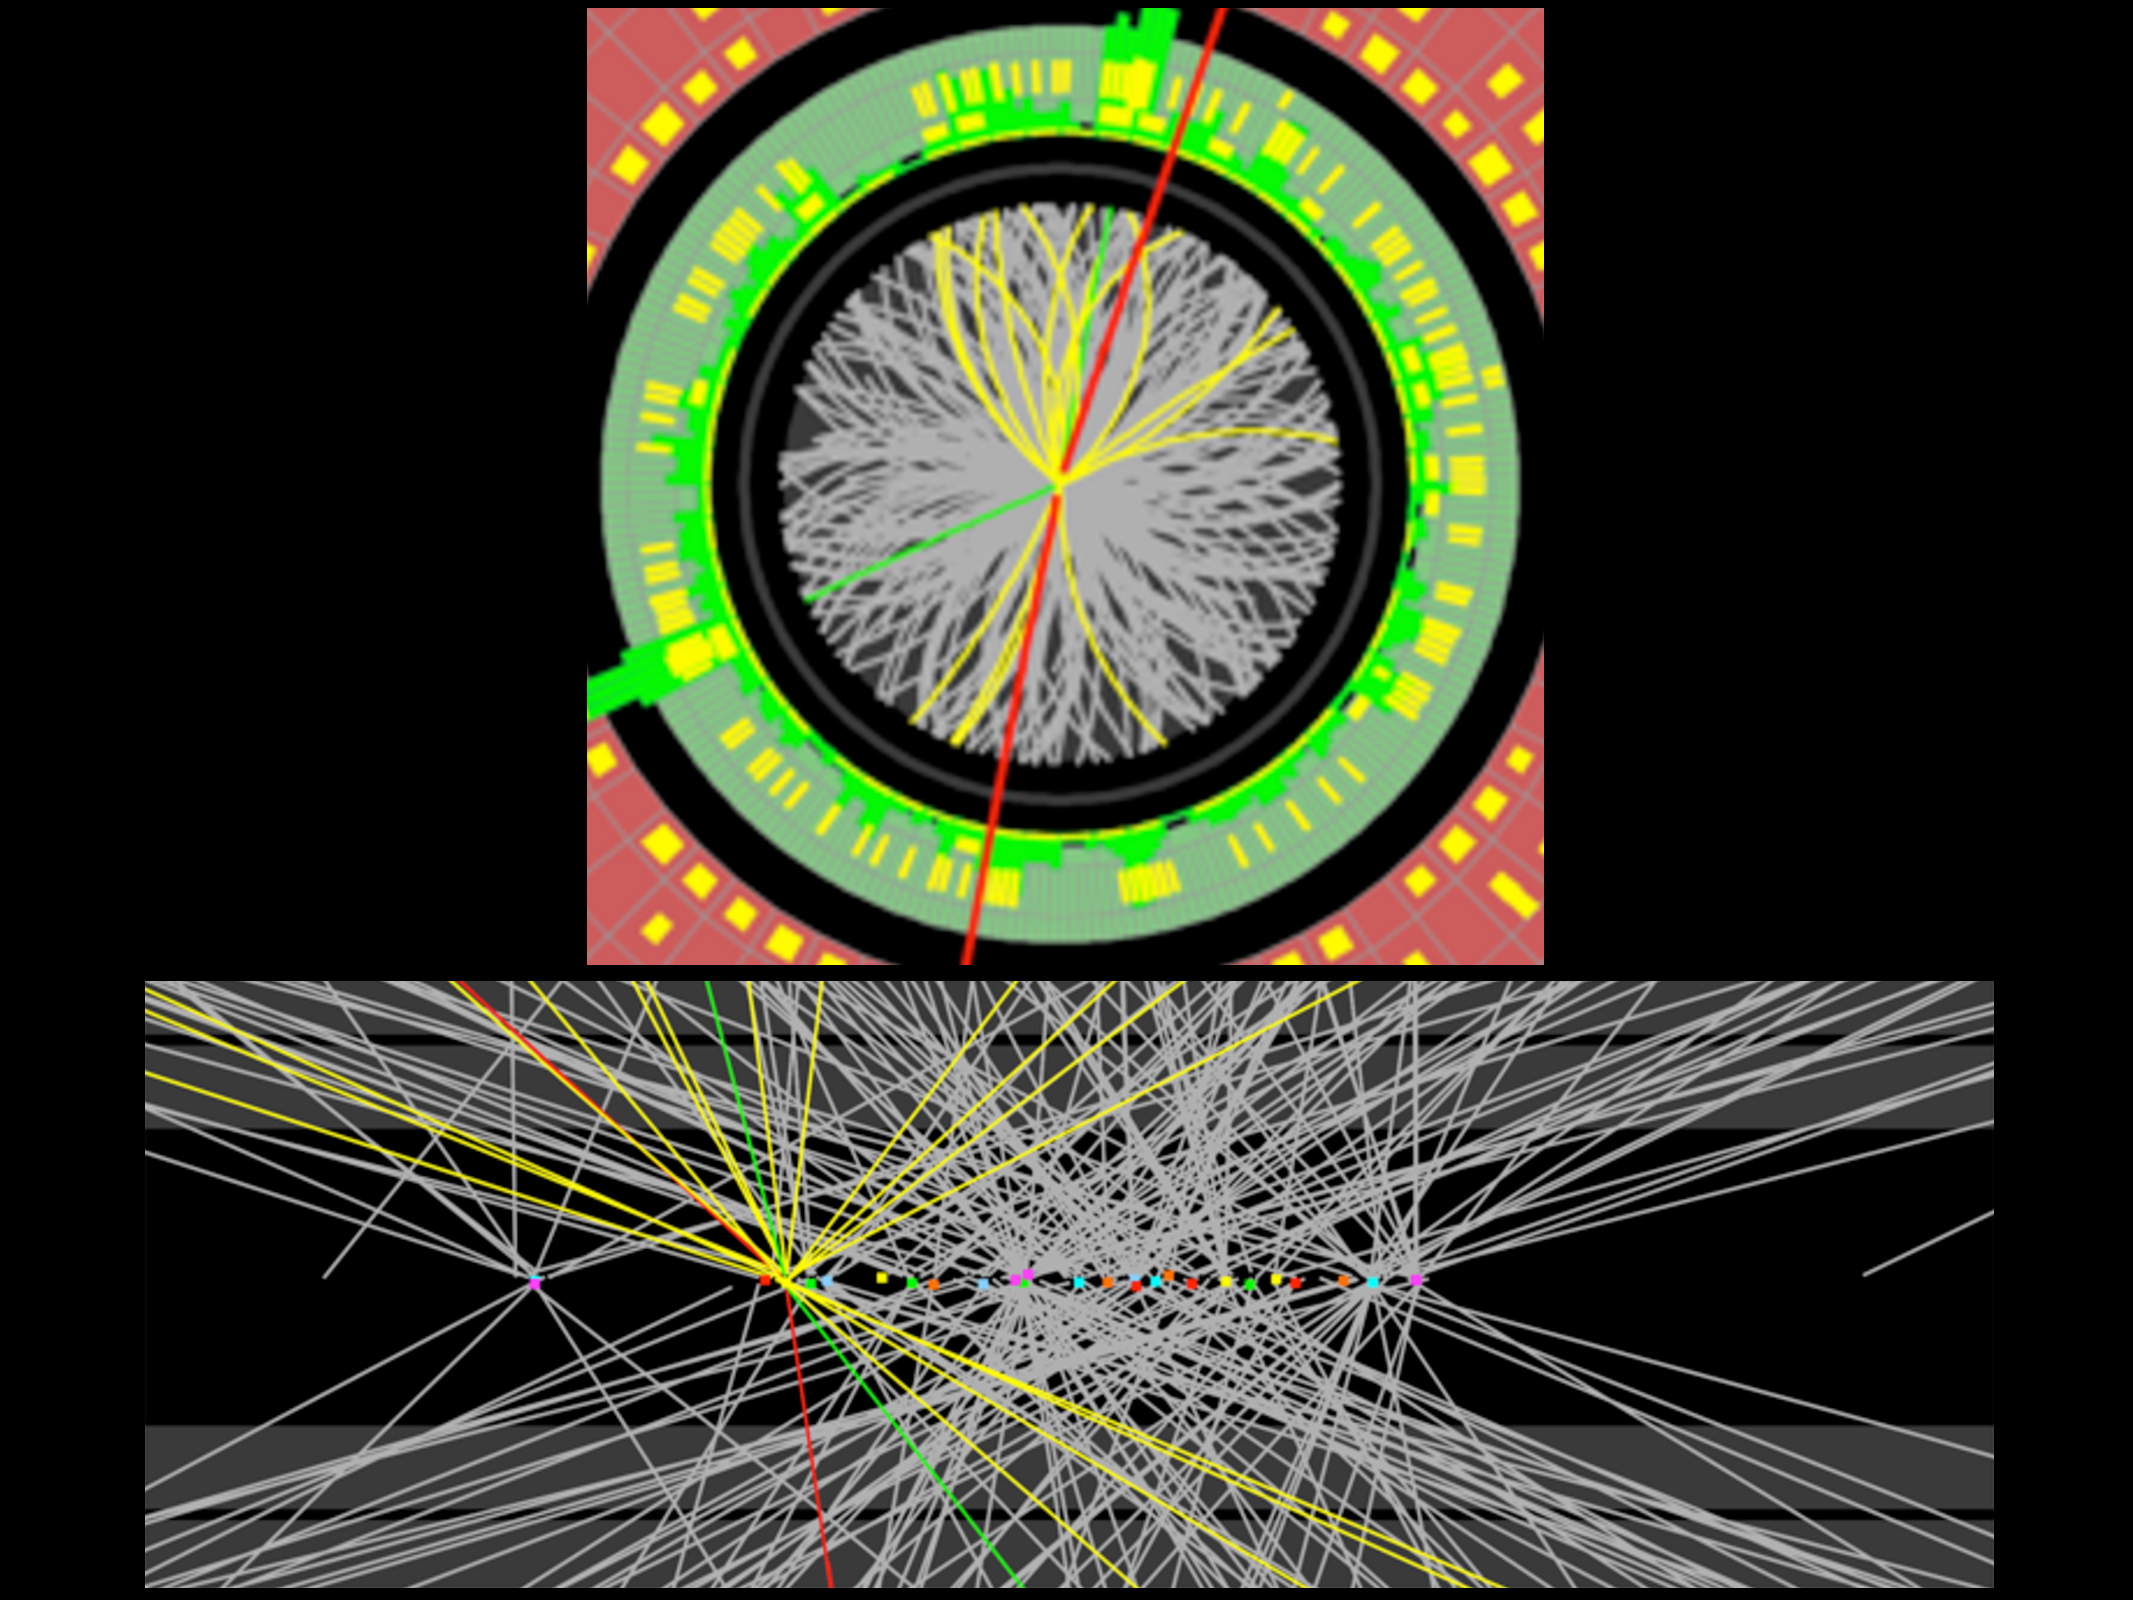
\includegraphics[width=0.725\textwidth]{./PileUp.pdf}
\ec

\clearpage

\underline{\textbf{Vacuum Fluctuations}}

QM+Spaceetime $\Rightarrow$ Anti-particles $\Rightarrow$ Vacuum is interesting place.

Because of QM, need to put in Energy to probe smaller distances.

\be
E\cdot t \sim E \cdot x \sim 1 \Rightarrow \rmt{Small distances} \Rightarrow \rmt{large E}
\ee

If $E >> 2m_2$ nothing stops you from making $e^+e^-$ pairs.

So operationally, should think of the vacuum as filled of particle-anti-particle pairs constantly coming in and out of existance:  

No meaningful sense in which the vacuum is empty.

\underline{Example 1}

\bc
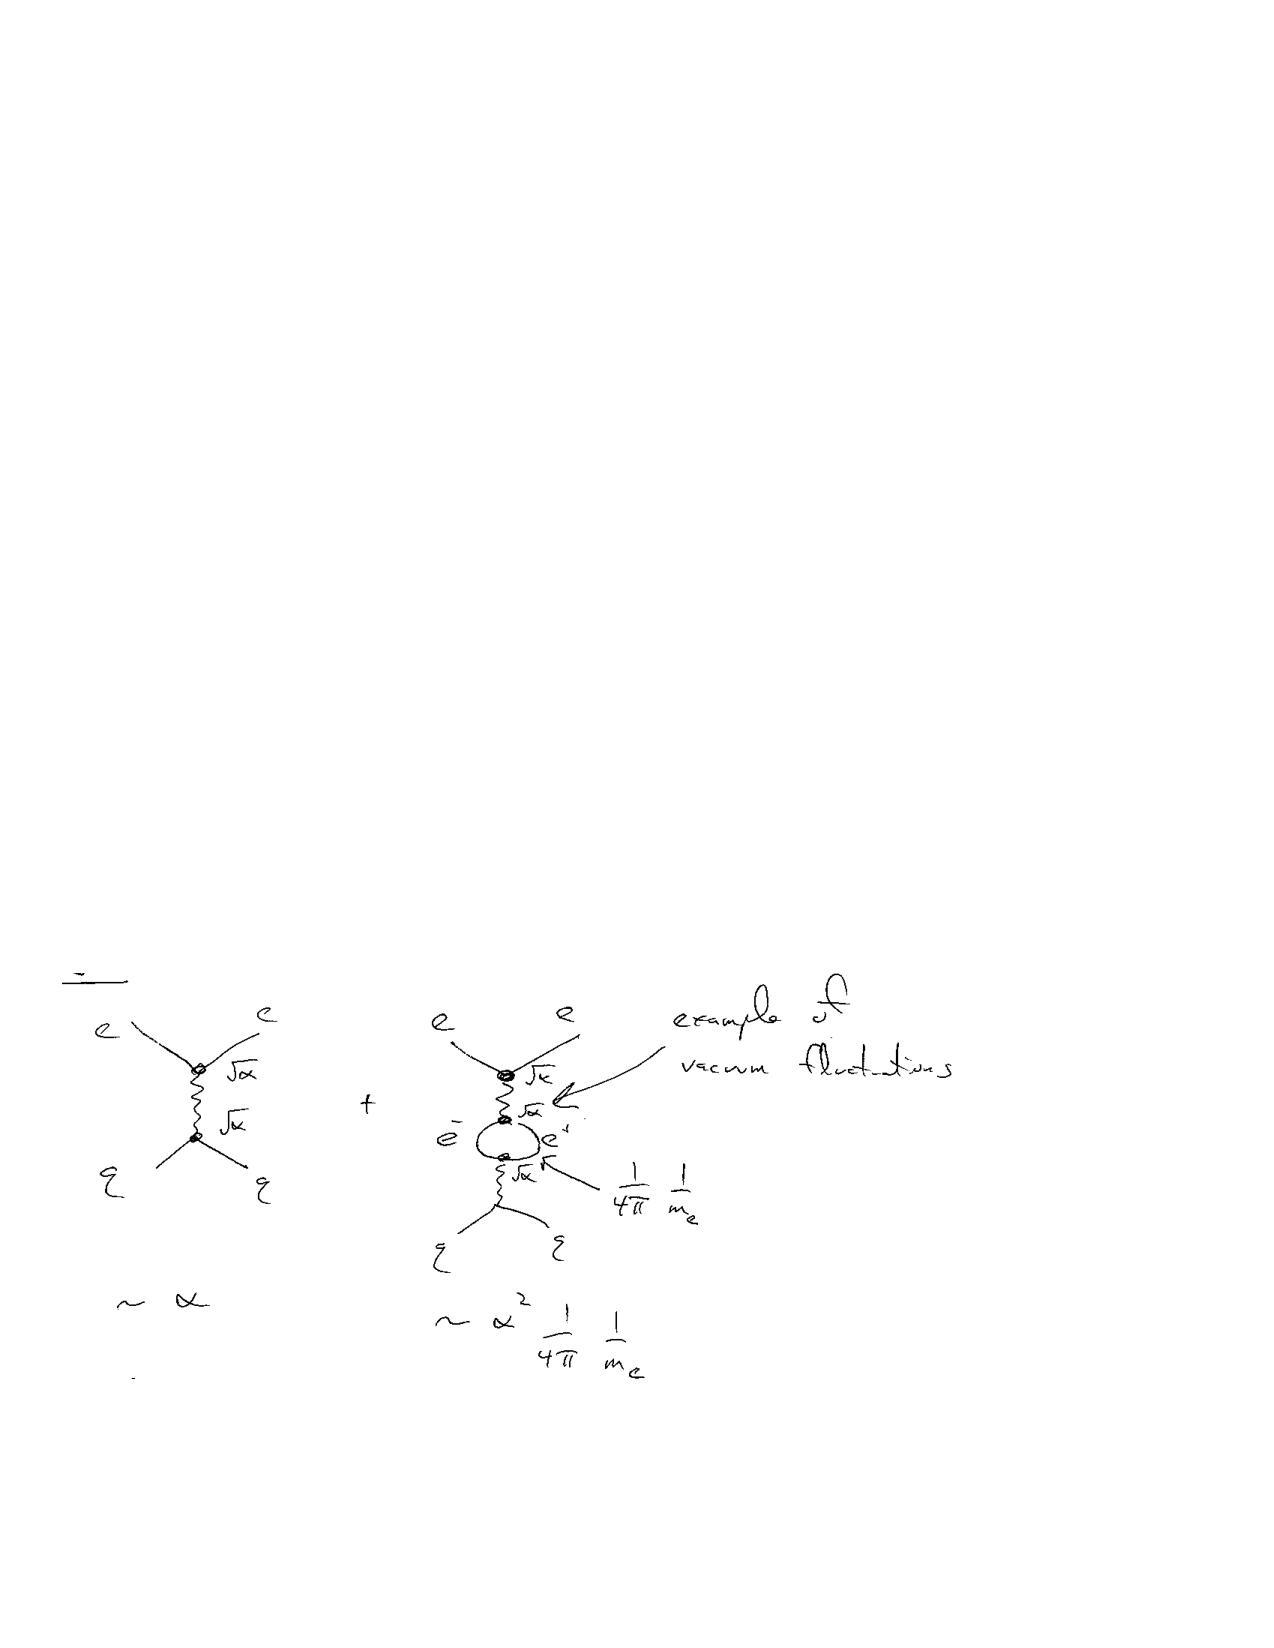
\includegraphics[width=\textwidth]{./VacuumFluctionations.pdf}
\ec

%\clearpage

\underline{Example 2}

\bc
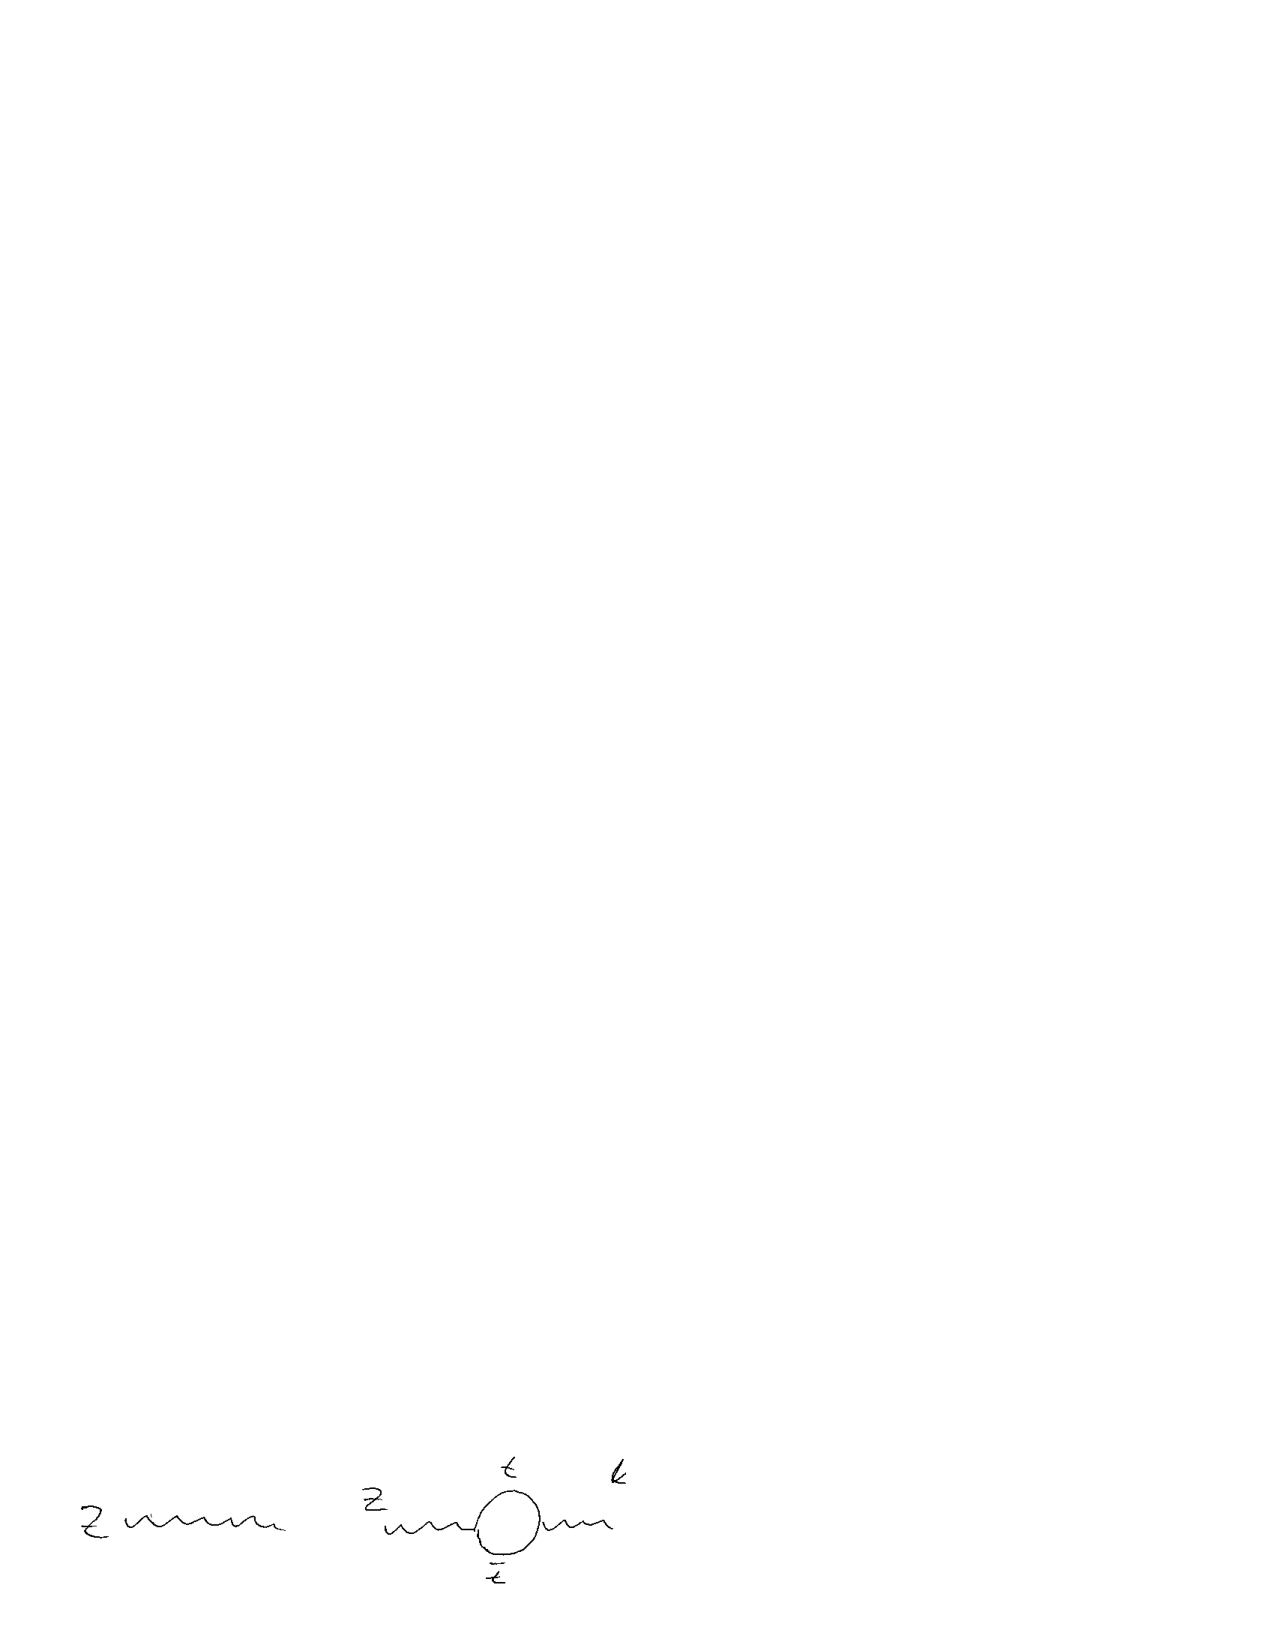
\includegraphics[width=0.5\textwidth]{./ZVacuumFluctionations.pdf}
\ec

Diagram gives a correction to the mass of the Z-boson from the top quark


\bc
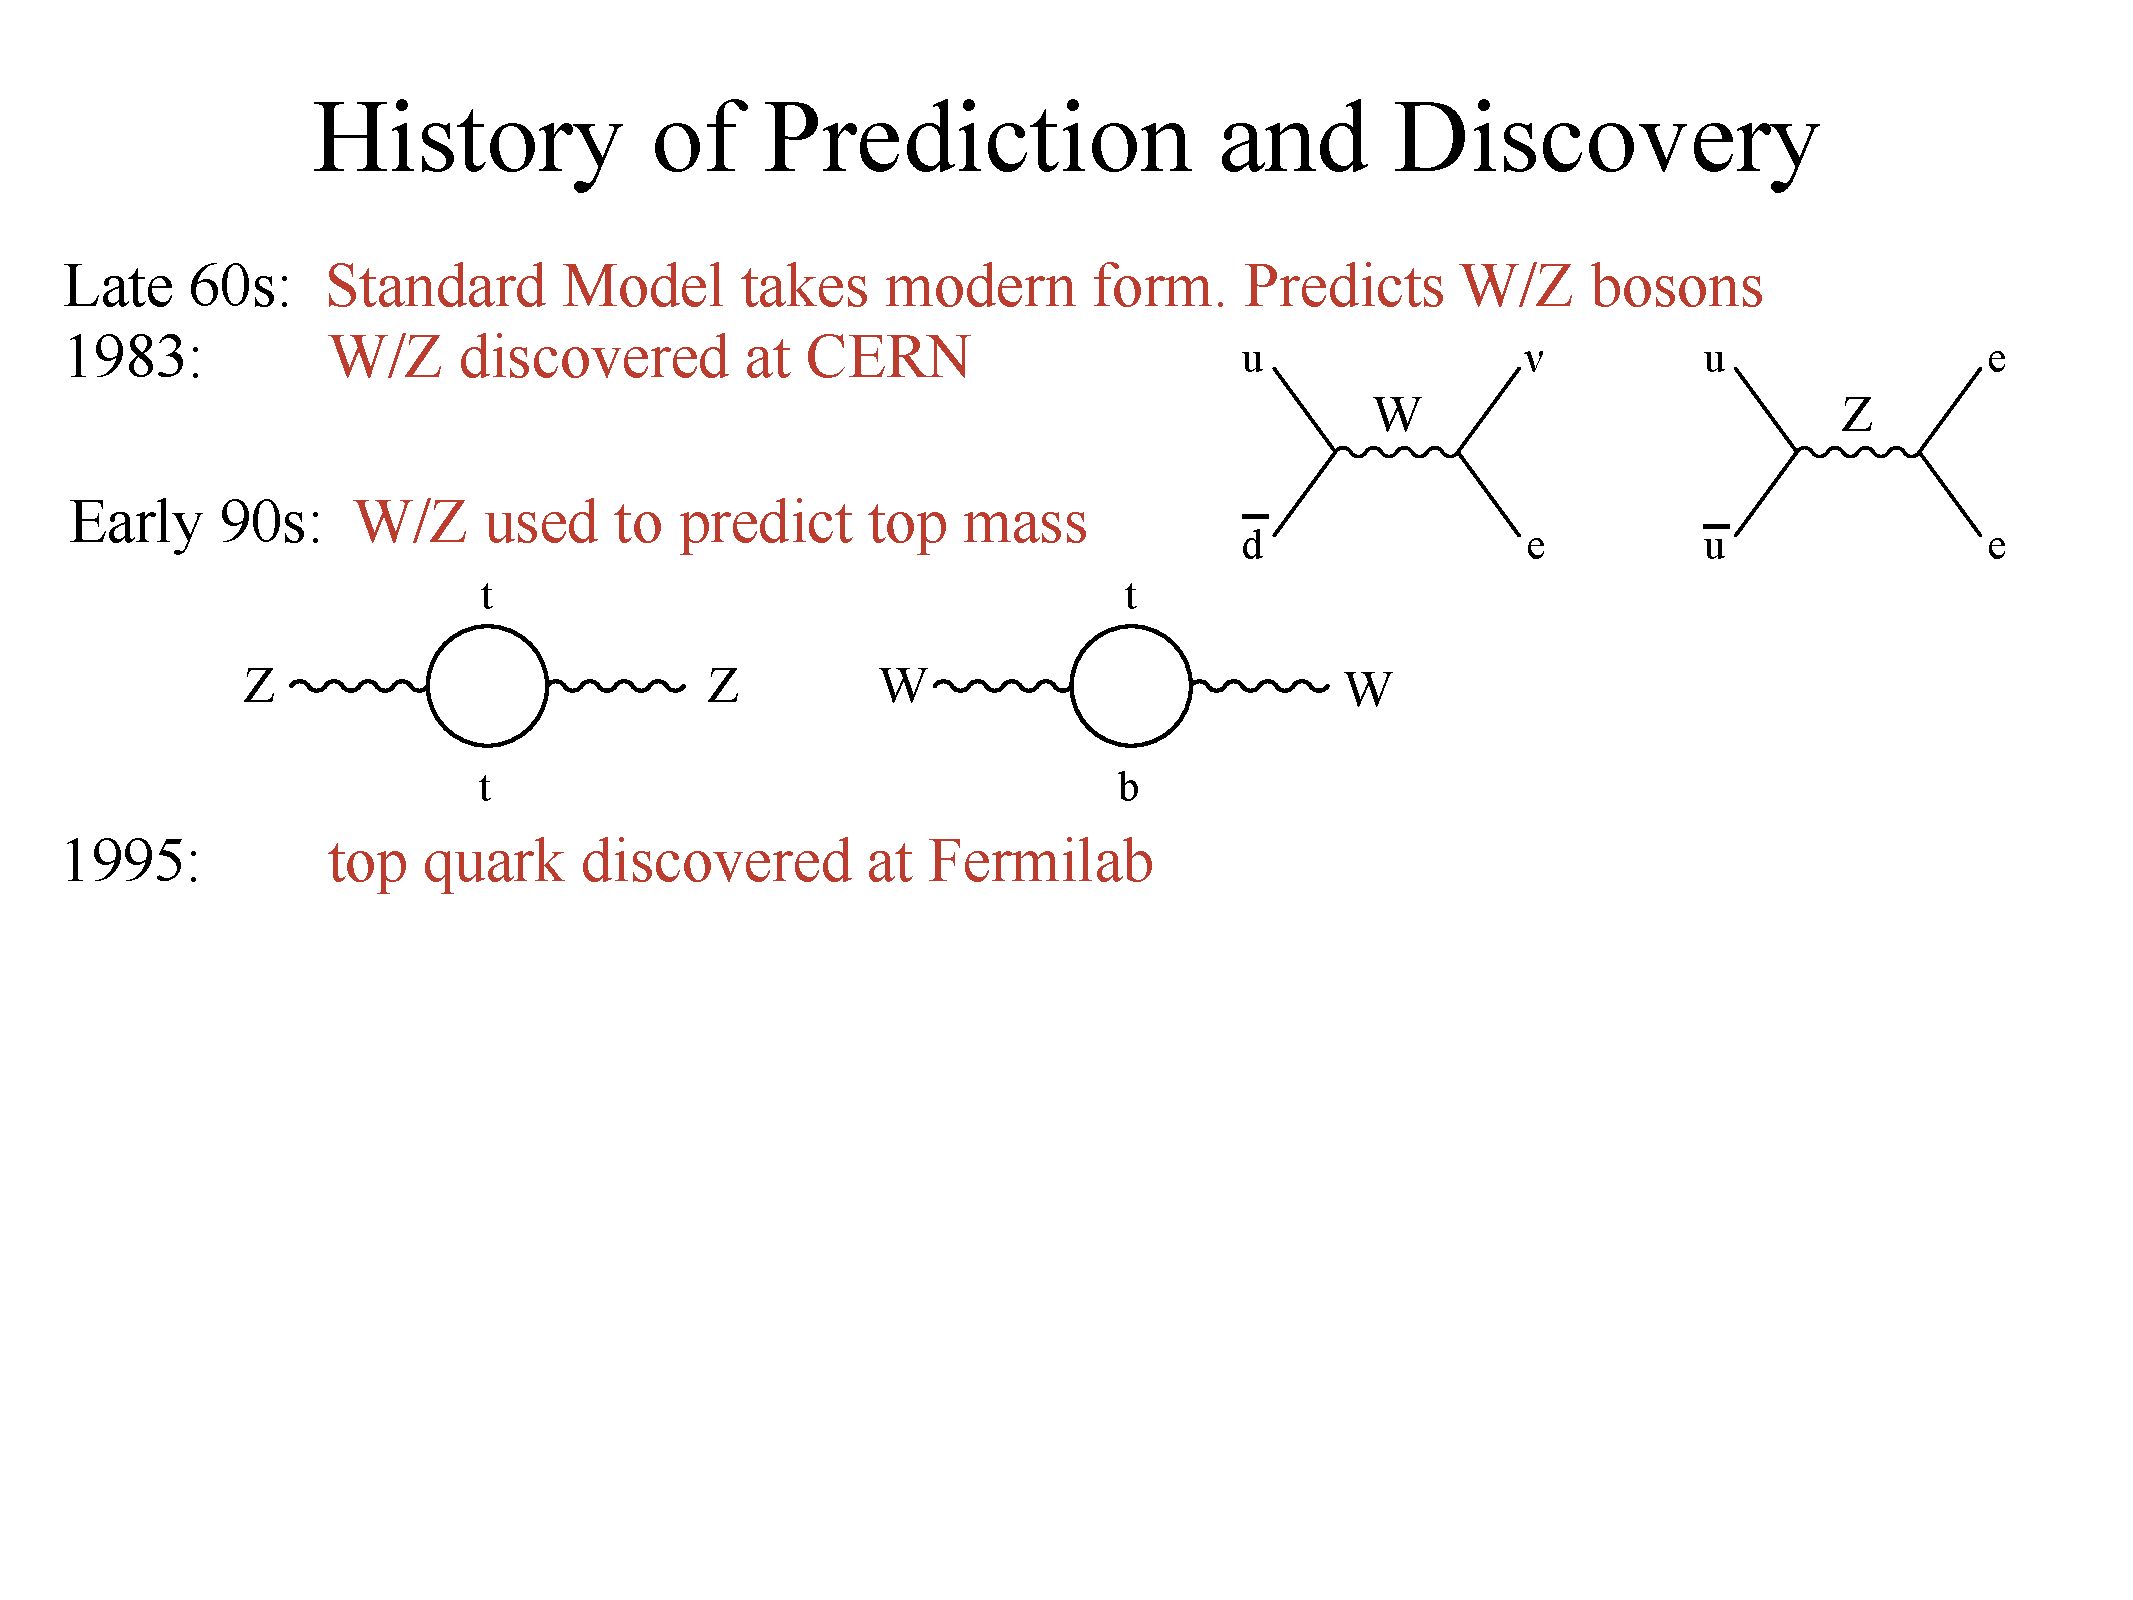
\includegraphics[width=1\textwidth]{./HistoryPredictionDiscovery.pdf}
\ec
\bc
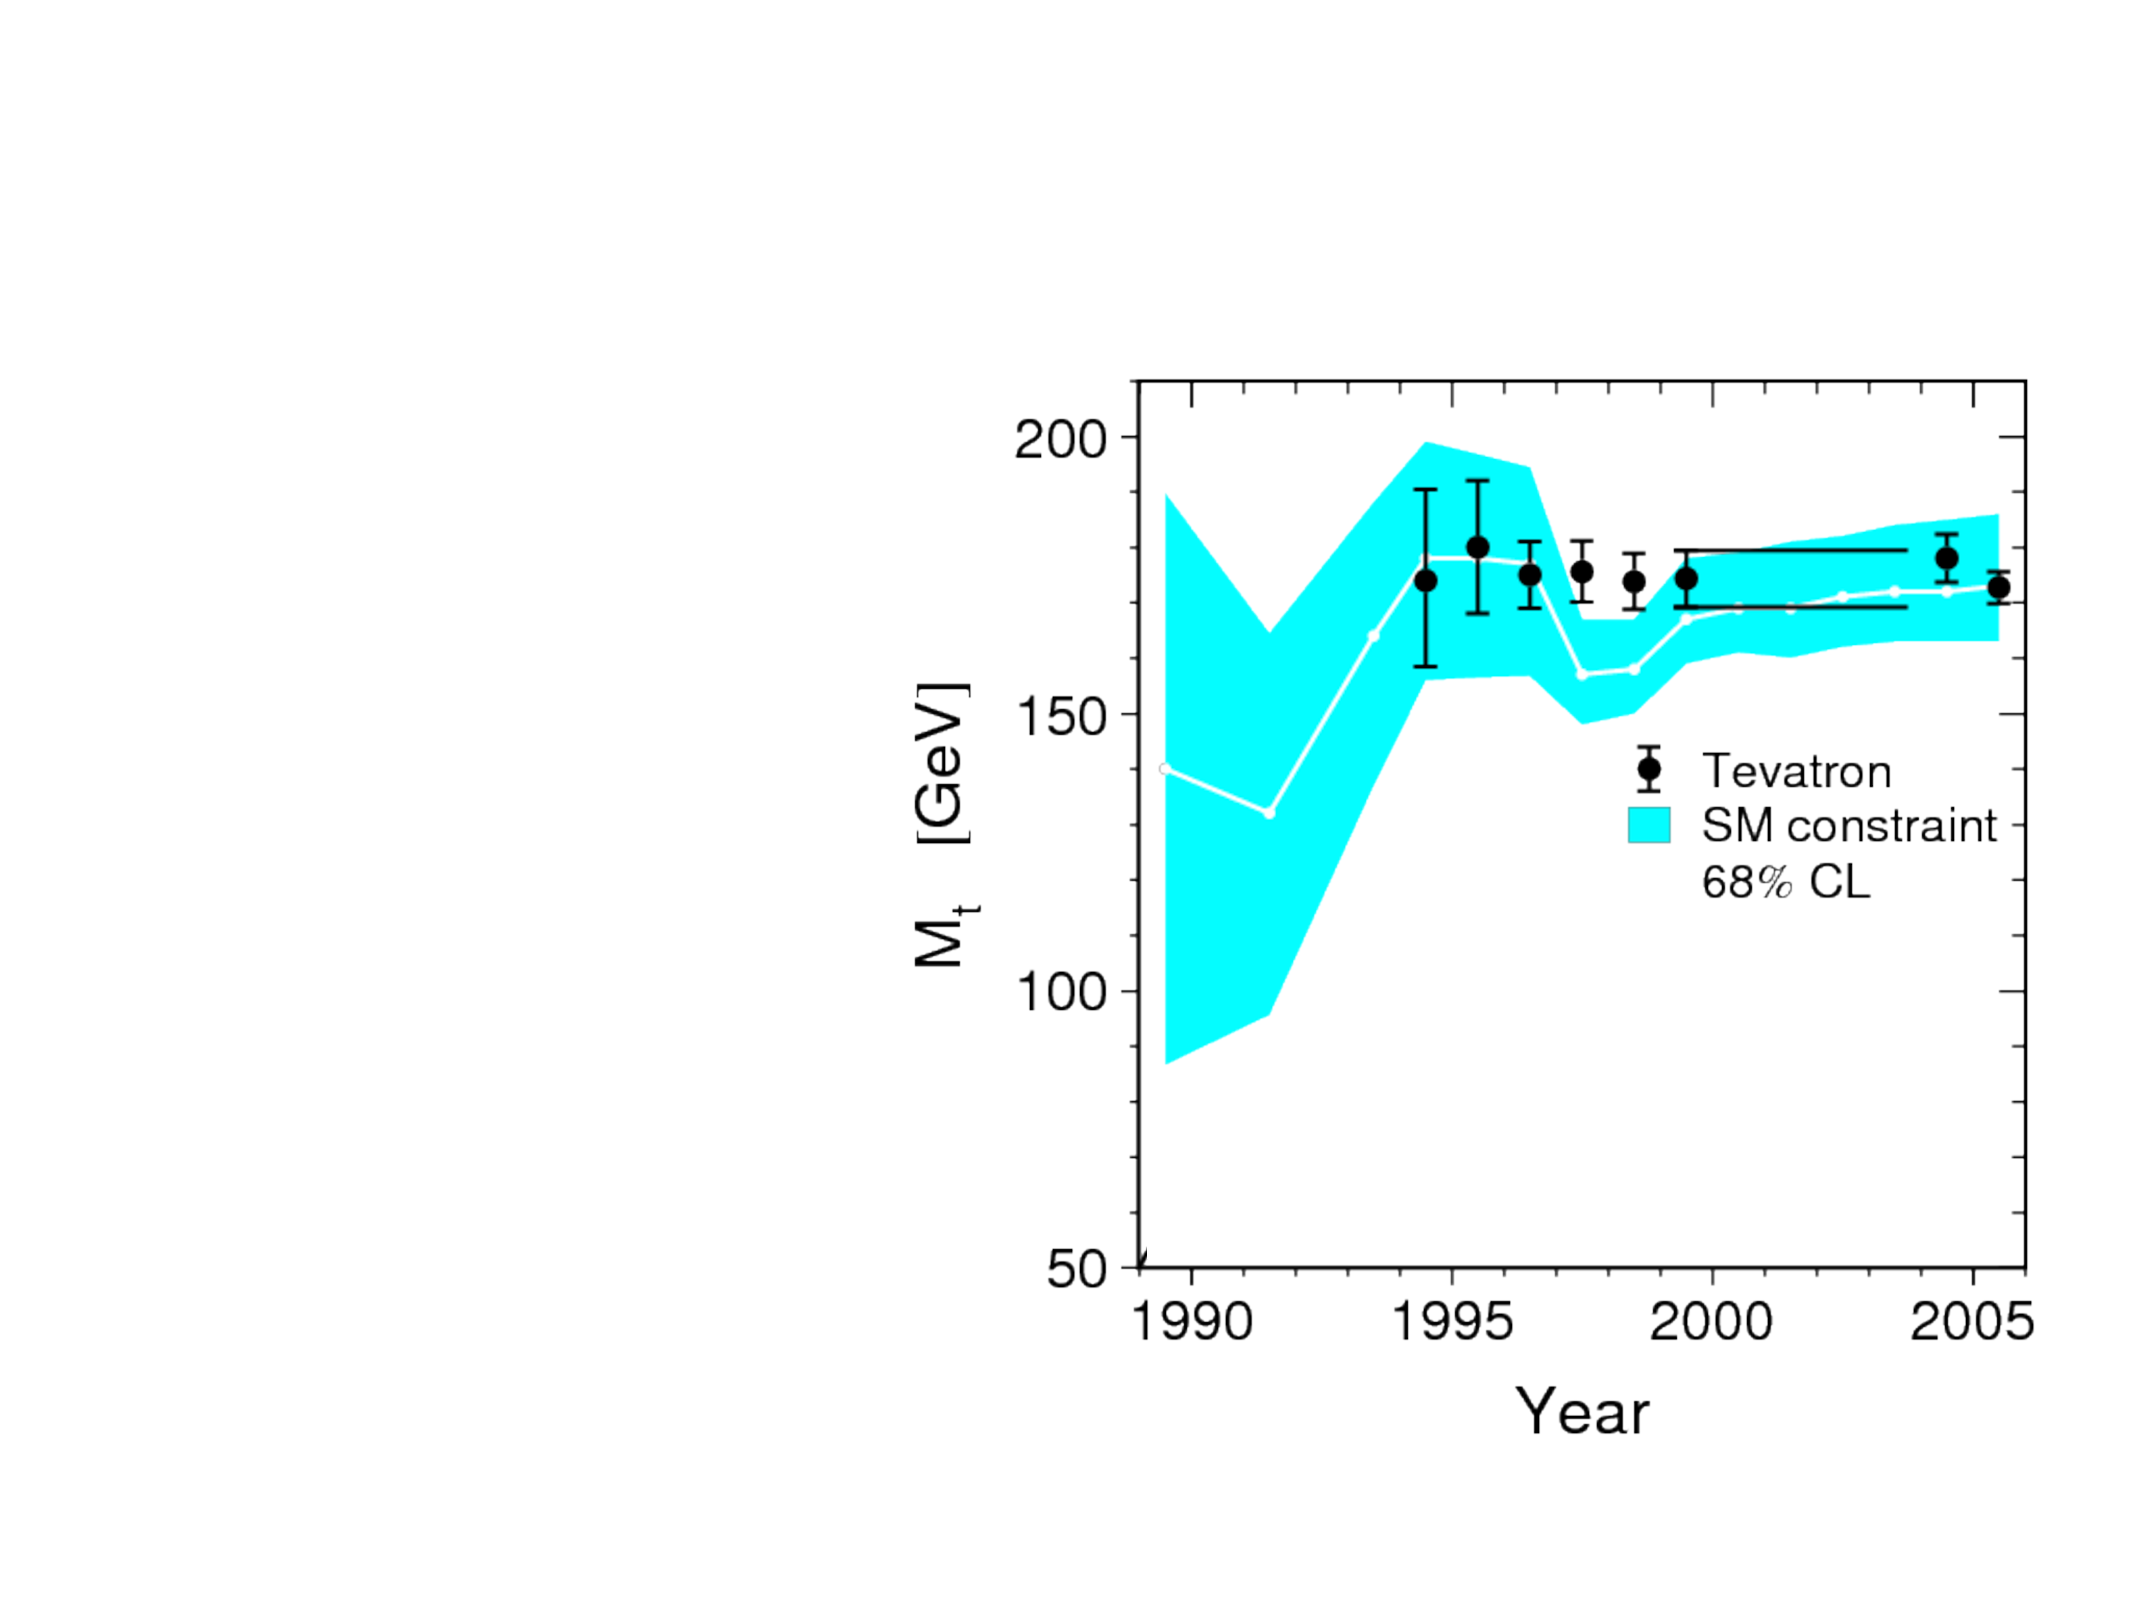
\includegraphics[width=0.4\textwidth]{./TopPrediction.pdf}
\ec
\bc
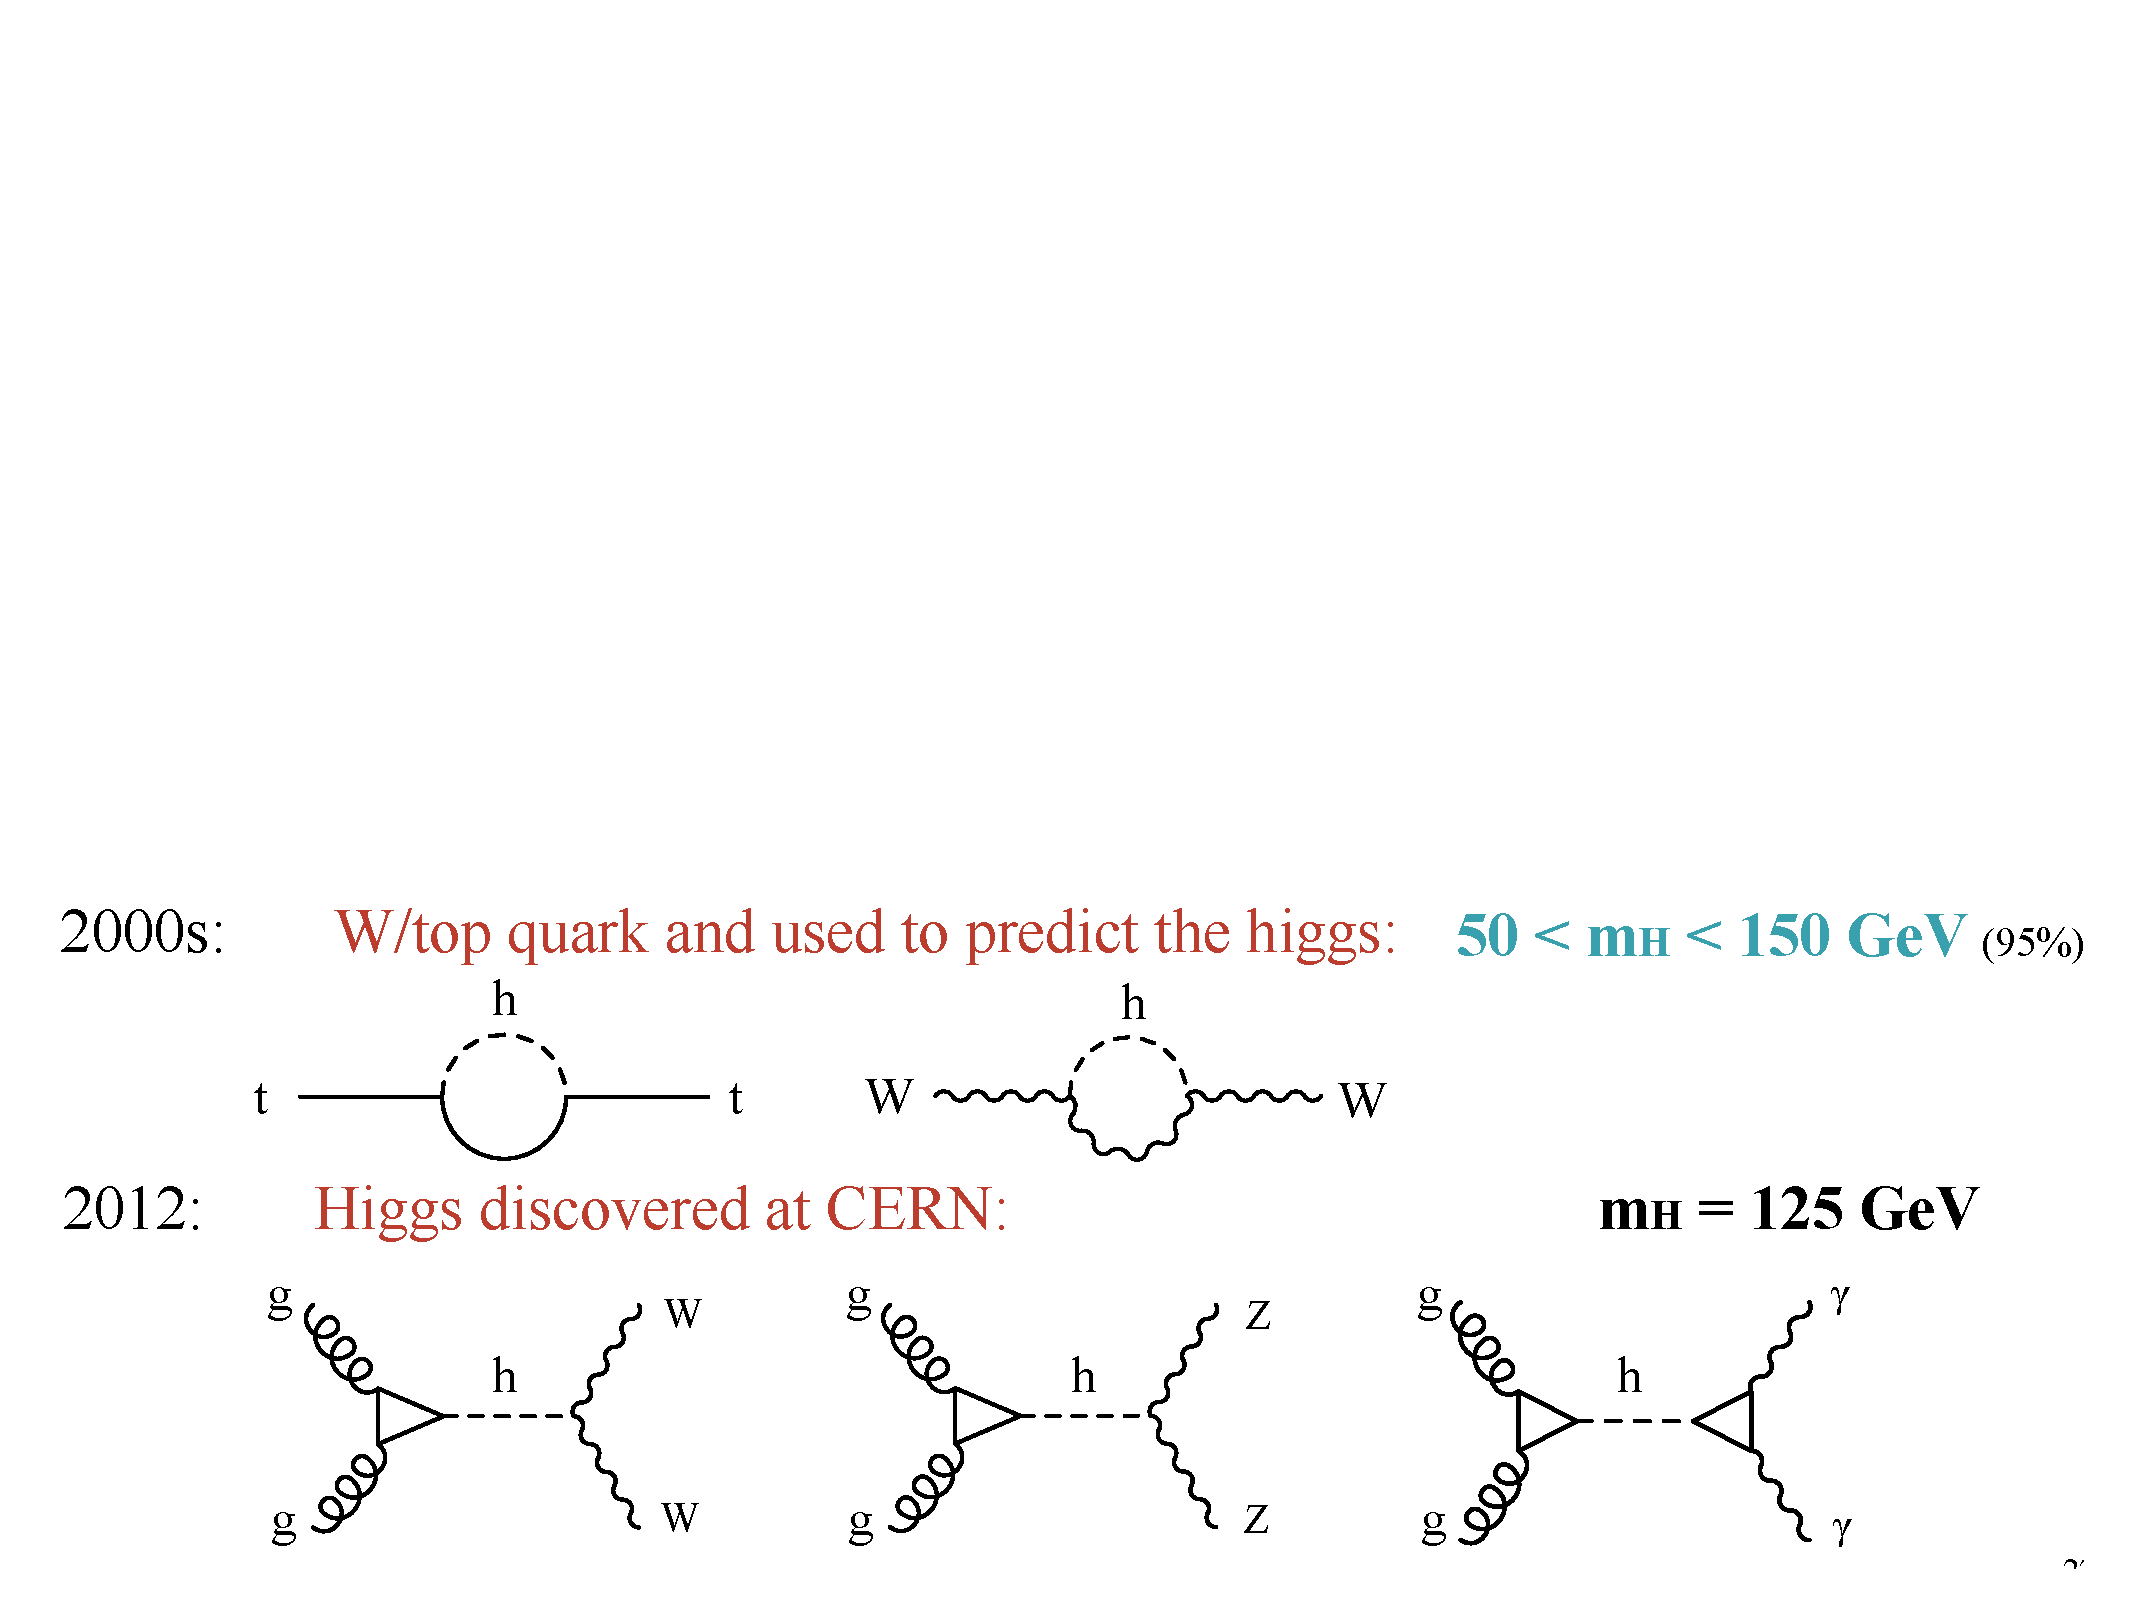
\includegraphics[width=1\textwidth]{./HistoryPart2.pdf}
\ec

These ``Quantum Corrections'' (Vacuum fluctuations) have \underline{observable} physical consequences.


Predicted the mass of the top quark and higgs boson before it was discovered. 

\lineacross

Forces all expressed in common language. 

At high energy $E \gtrsim  m_{W,Z}$, first time we see that all forces described in same basic way.
\bc
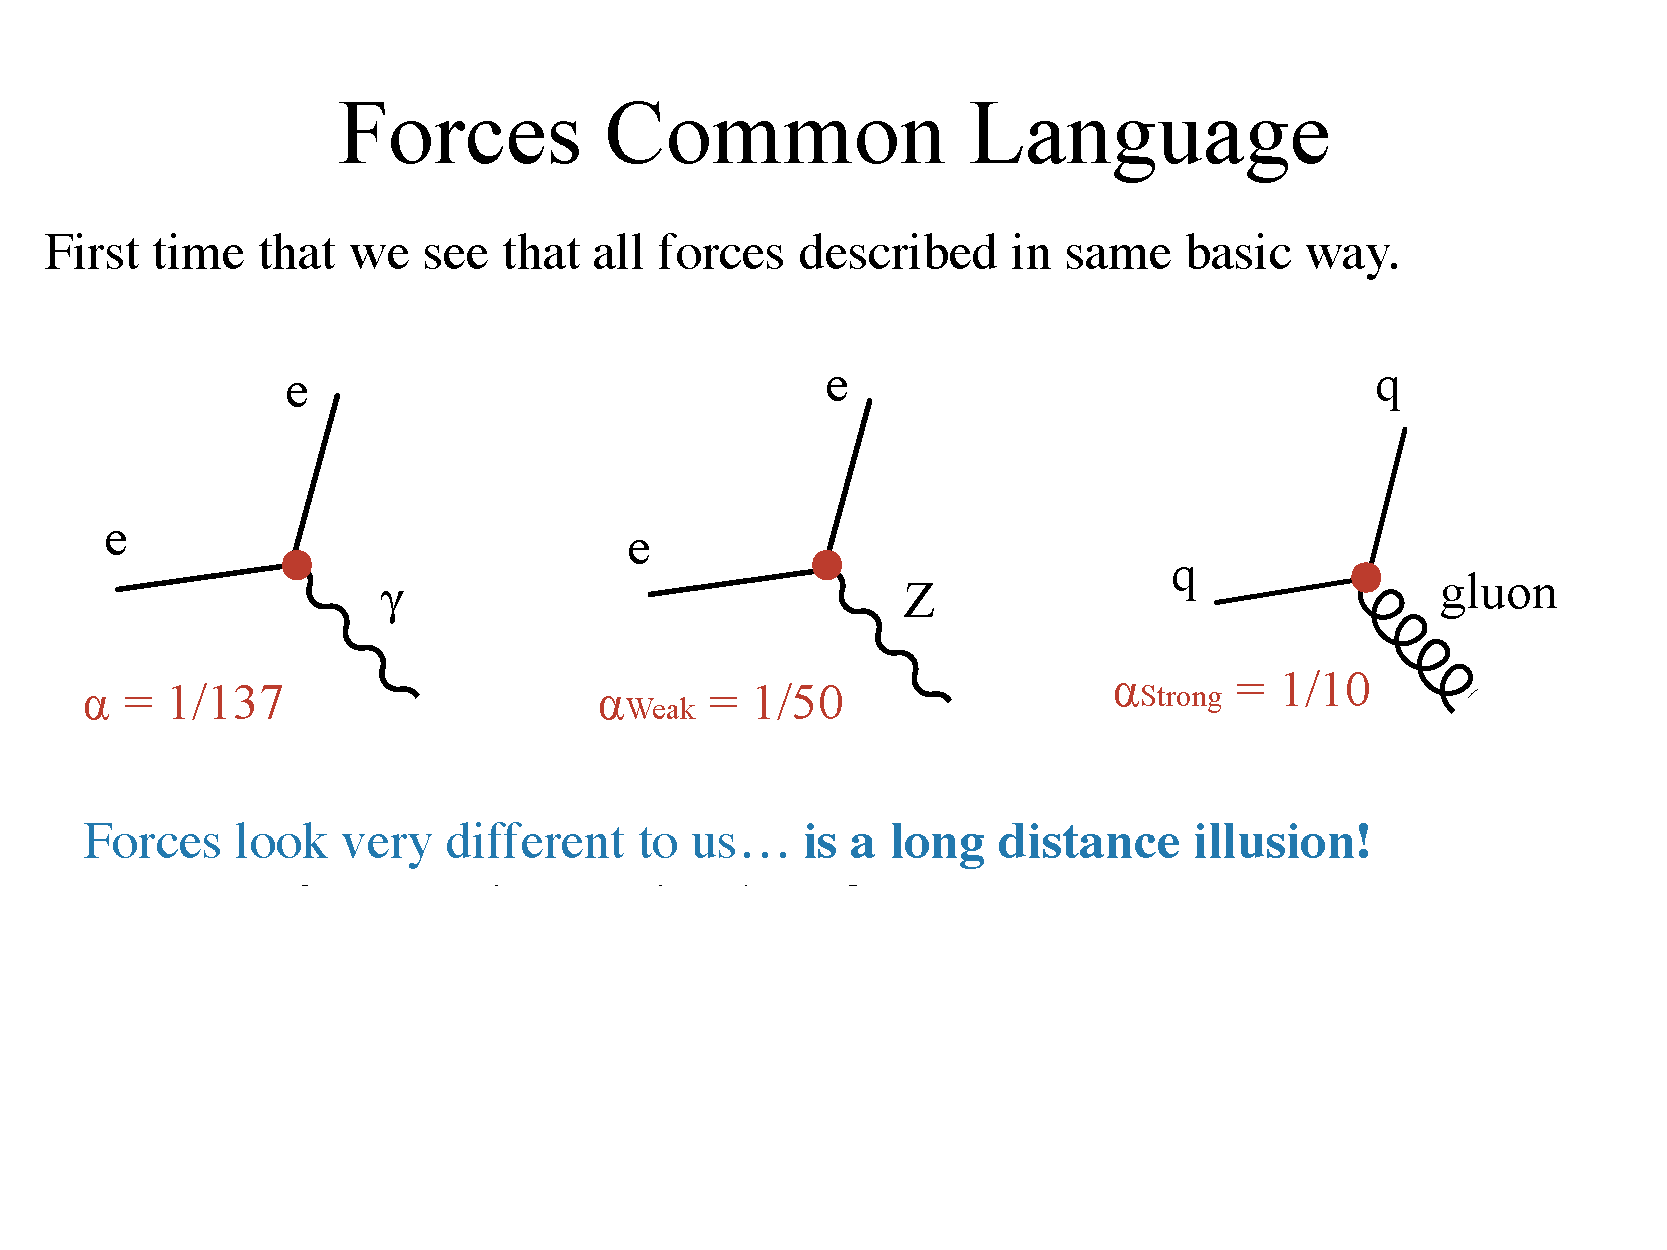
\includegraphics[width=1\textwidth]{./ForcesCommon.pdf}
\ec
This is the real reason we build colliders!  See basic underlying symmetry.


We already talked about this for the weak interaction. ($m_W$ and $m_Z >> 0$ cuts of the range of the force) 


Now lets look at why the strong interaction looks so different...

\clearpage

Imagine you wanted to measure the EM strength vs distance. 
\bc
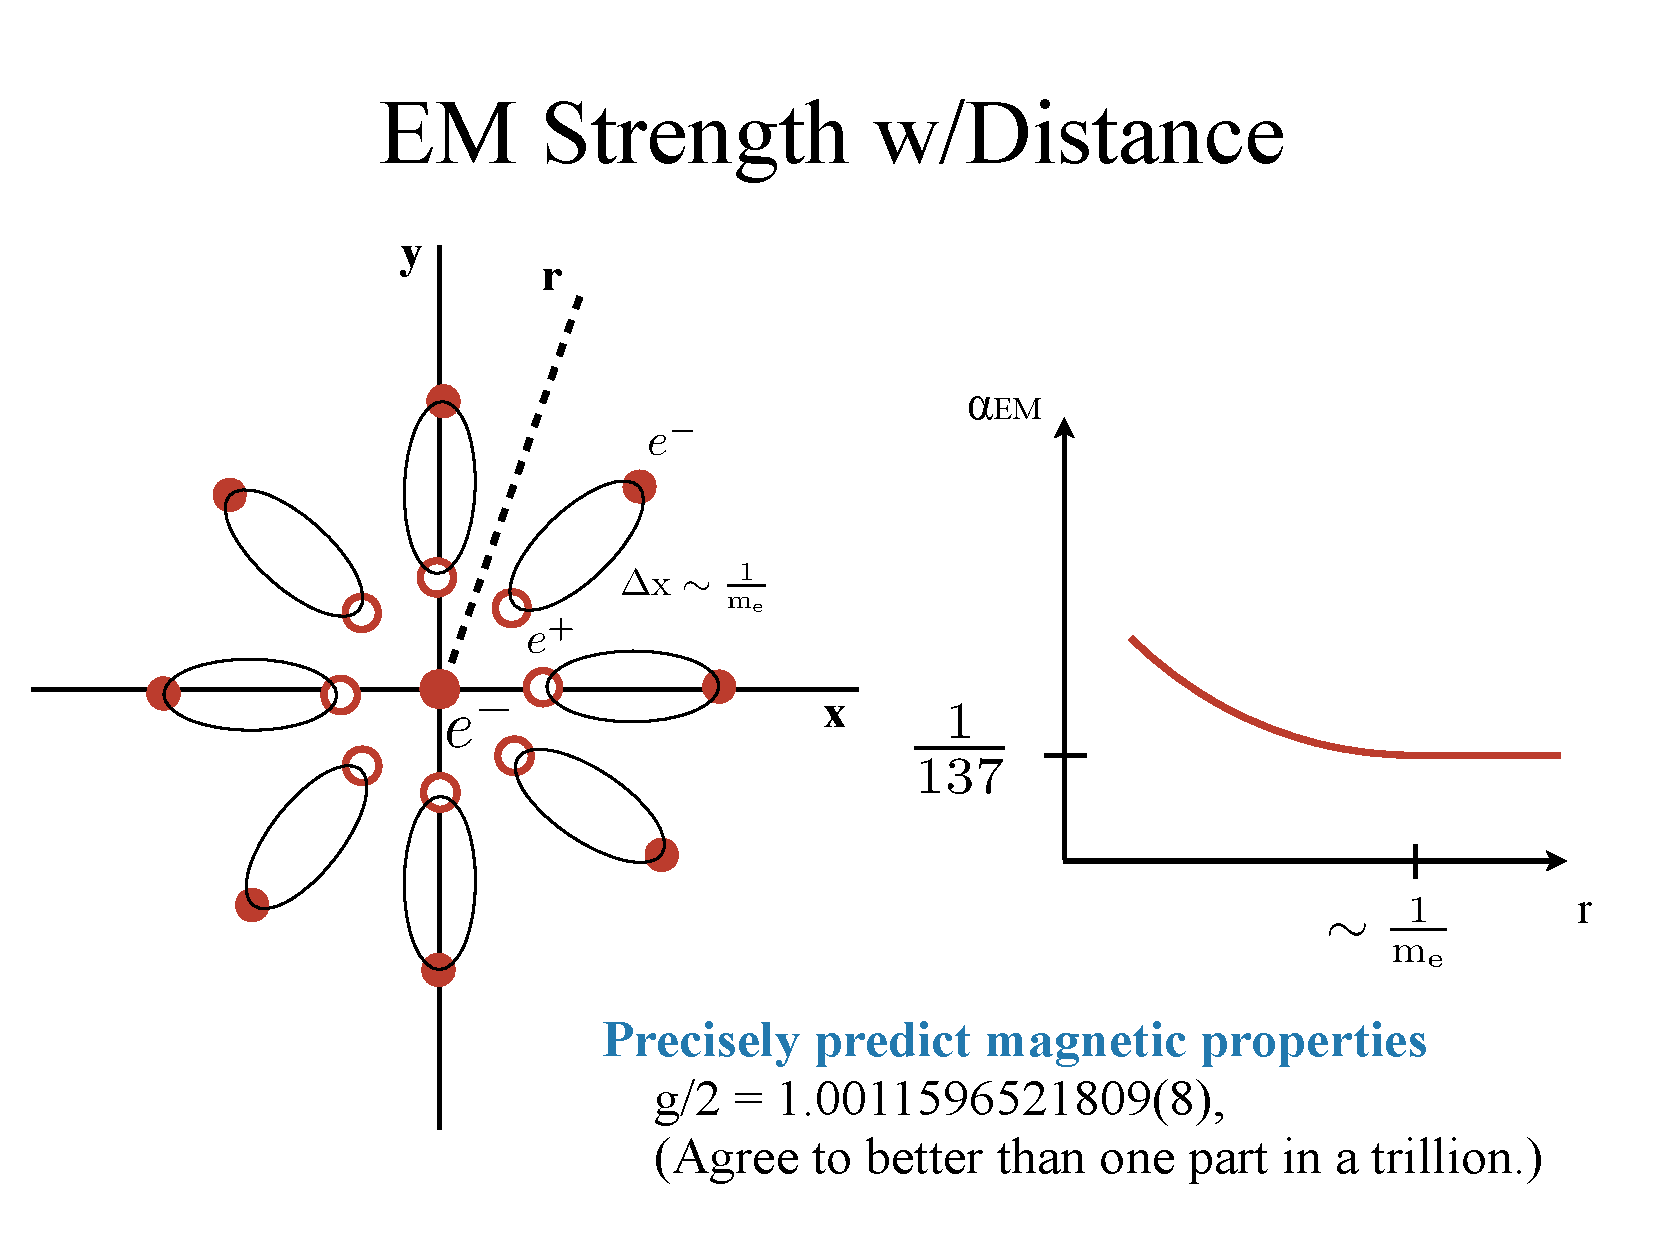
\includegraphics[width=1\textwidth]{./EMStrenghtVsDistance.pdf}
\ec
$\alpha$ increases because you are ``seeing'' more of the bare electron charge.

\lineacross

\clearpage

Same game with the Strong Interaction
\bc
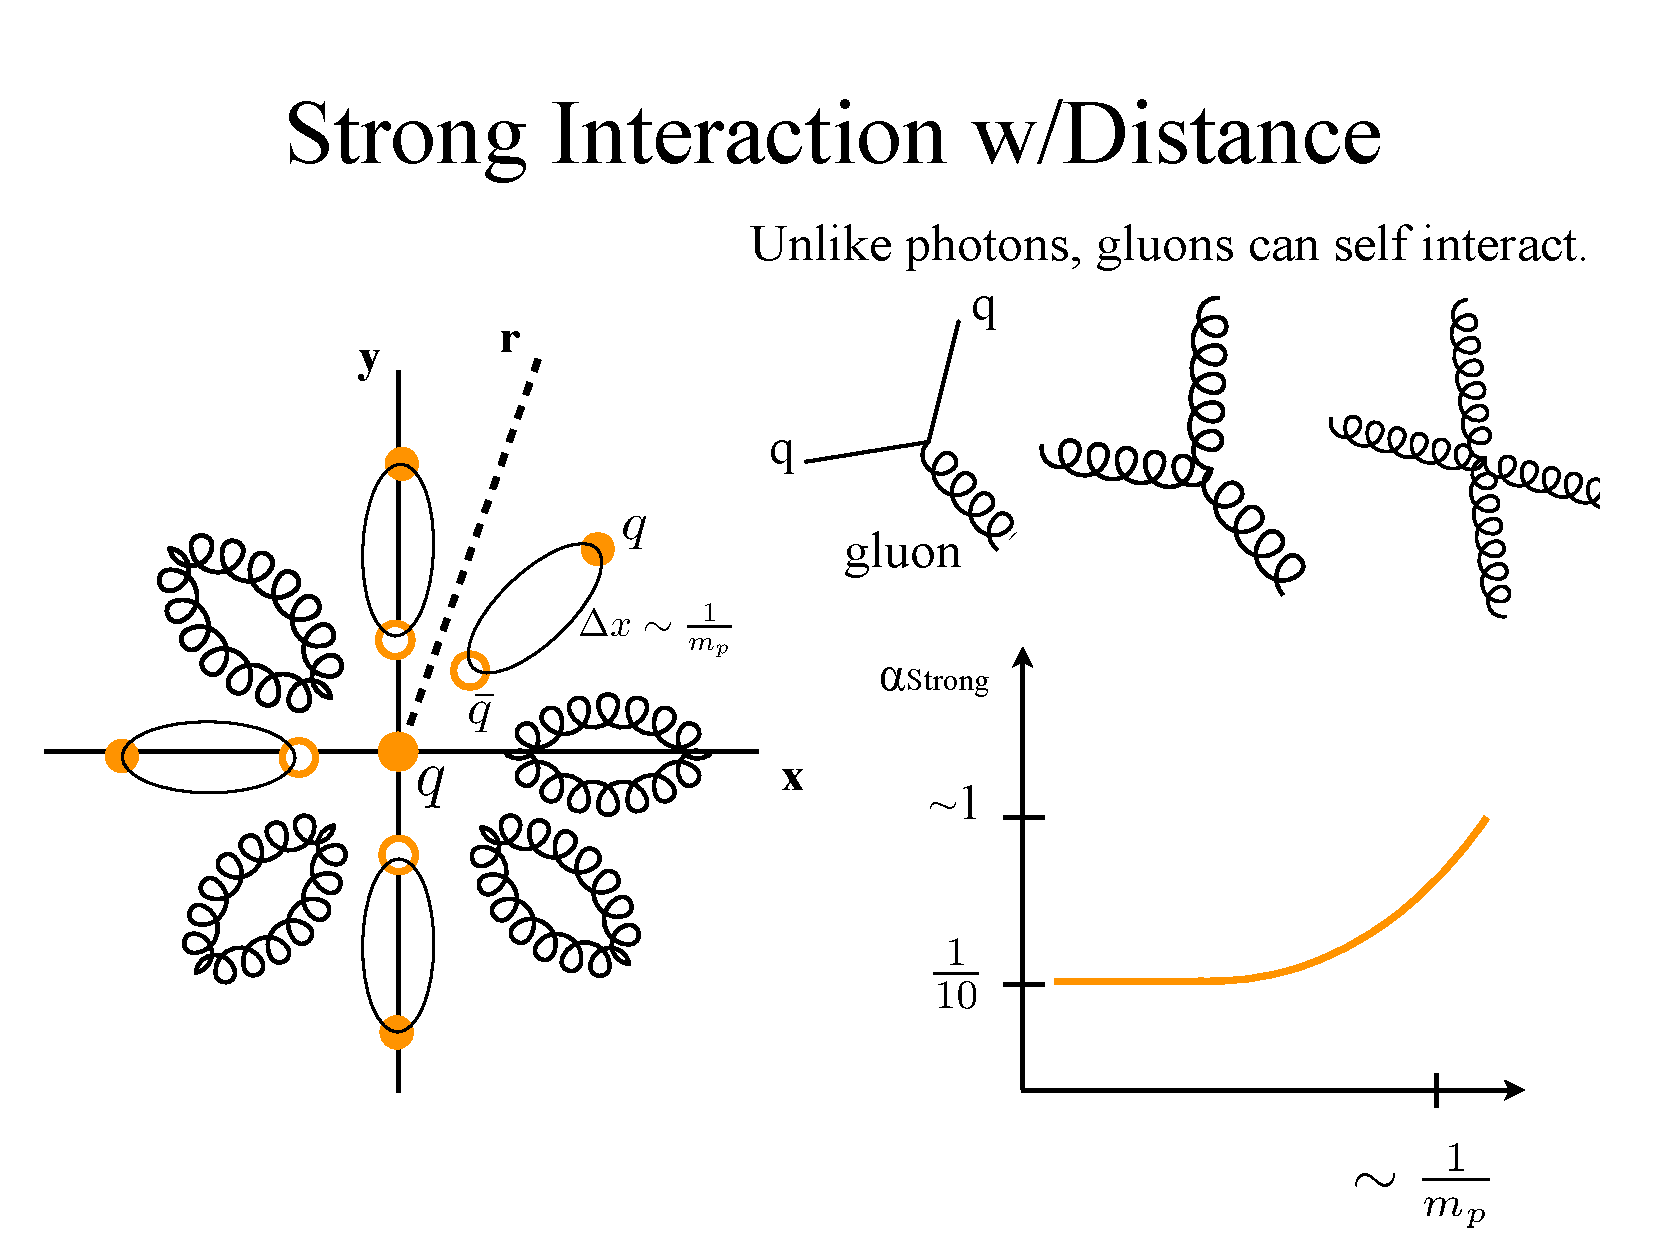
\includegraphics[width=1\textwidth]{./StrongInteractionVsDistance.pdf}
\ec

Increase is an ``accident'' depends on the number of colors, the number of quarks and gauge group.
\bc
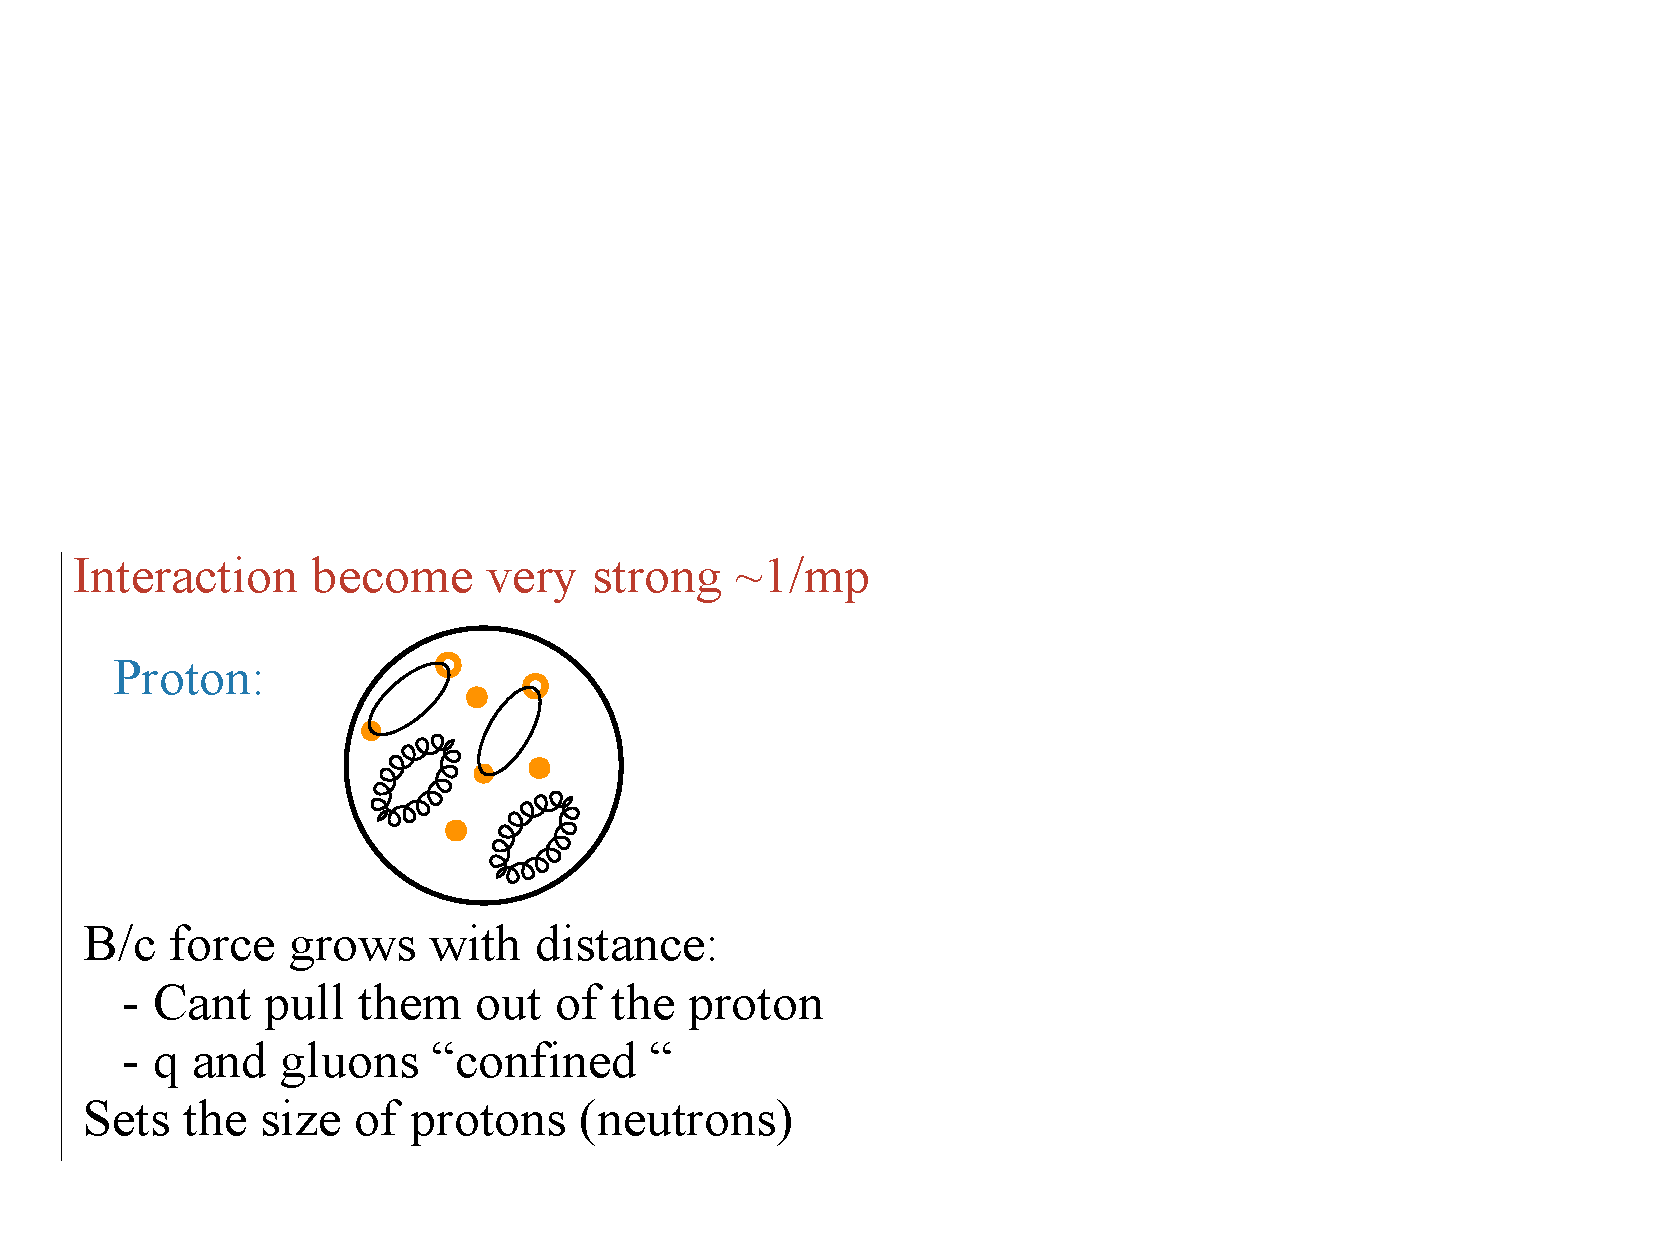
\includegraphics[width=0.45\textwidth]{./Proton.pdf}
\ec

  


}
\end{document}


